% Judul dokumen
\title{Buku Tugas Akhir ITS}
\author{Dafa Fidini Asqav}

% Pengaturan ukuran teks dan bentuk halaman dua sisi
\documentclass[12pt,twoside]{report}

% Pengaturan ukuran halaman dan margin
\usepackage[a4paper,top=30mm,left=30mm,right=20mm,bottom=25mm]{geometry}

% Pengaturan ukuran spasi
\usepackage[singlespacing]{setspace}

% Pengaturan format bahasa
\usepackage[indonesian]{babel}

% Pengaturan detail pada file PDF
\usepackage[pdfauthor={\@author},bookmarksnumbered,pdfborder={0 0 0}]{hyperref}

% Pengaturan jenis karakter
\usepackage[utf8]{inputenc}

% Pengaturan pewarnaan
\usepackage[table,xcdraw]{xcolor}

% Pengaturan kutipan artikel
\usepackage{natbib}

% Package lainnya
\usepackage{changepage}
\usepackage{enumitem}
\usepackage{eso-pic}
\usepackage{etoolbox}
\usepackage{graphicx}
\usepackage{lipsum}
\usepackage{lmodern}
\usepackage{longtable}
\usepackage{tabularx}
\usepackage{wrapfig}
\usepackage{float}
\usepackage{amsmath,amssymb,amsfonts}
\usepackage{multirow}


% Definisi untuk "Hati ini sengaja dikosongkan"
\patchcmd{\cleardoublepage}{\hbox{}}{
  \thispagestyle{empty}
  \vspace*{\fill}
  \begin{center}\textit{[Halaman ini sengaja dikosongkan]}\end{center}
  \vfill}{}{}

% Pengaturan penomoran halaman
\usepackage{fancyhdr}
\fancyhf{}
\renewcommand{\headrulewidth}{0pt}
\pagestyle{fancy}
\fancyfoot[LE,RO]{\thepage}
\patchcmd{\chapter}{plain}{fancy}{}{}
\patchcmd{\chapter}{empty}{plain}{}{}

% Pengaturan format judul bab
\usepackage{titlesec}
\titleformat{\chapter}[display]{\bfseries\Large}{BAB \centering\Roman{chapter}}{0ex}{\vspace{0ex}\centering}
\titleformat{\section}{\bfseries\large}{\MakeUppercase{\thesection}}{1ex}{\vspace{1ex}}
\titleformat{\subsection}{\bfseries\large}{\MakeUppercase{\thesubsection}}{1ex}{}
\titleformat{\subsubsection}{\bfseries\large}{\MakeUppercase{\thesubsubsection}}{1ex}{}
\titlespacing{\chapter}{0ex}{0ex}{4ex}
\titlespacing{\section}{0ex}{1ex}{0ex}
\titlespacing{\subsection}{0ex}{0.5ex}{0ex}
\titlespacing{\subsubsection}{0ex}{0.5ex}{0ex}

% Pengaturan format potongan kode
\usepackage{listings}
\definecolor{comment}{RGB}{0,128,0}
\definecolor{string}{RGB}{255,0,0}
\definecolor{keyword}{RGB}{0,0,255}
\lstdefinestyle{codestyle}{
  commentstyle=\color{comment},
  stringstyle=\color{string},
  keywordstyle=\color{keyword},
  basicstyle=\footnotesize\ttfamily,
  numbers=left,
  numberstyle=\tiny,
  numbersep=5pt,
  frame=lines,
  breaklines=true,
  prebreak=\raisebox{0ex}[0ex][0ex]{\ensuremath{\hookleftarrow}},
  showstringspaces=false,
  upquote=true,
  tabsize=2,
}
\lstset{style=codestyle}

% Isi keseluruhan dokumen
\begin{document}

  % Sampul luar Bahasa Indonesia
  \newcommand\covercontents{sampul/konten-id.tex}
  \AddToShipoutPictureBG*{
  \AtPageLowerLeft{
    % Ubah nilai berikut jika posisi horizontal background tidak sesuai
    \hspace{-3.5mm}

    % Ubah nilai berikut jika posisi vertikal background tidak sesuai
    \raisebox{0mm}{
      
\includegraphics[width=\paperwidth,height=\paperheight]{sampul/gambar/sampul-luar2.png}
    }
  }
}

% Menyembunyikan nomor halaman
\thispagestyle{empty}

% Pengaturan margin untuk menyesuaikan konten sampul
\newgeometry{
  top=55mm,
  left=30mm,
  right=20mm,
  bottom=25mm
}

\begin{flushleft}
  % Pemilihan font sans serif
  \sffamily

  % Pemilihan warna font putih
  \color{white}

  % Pemilihan font bold
  % \fontseries{bx}
  \selectfont

  \input{\covercontents}

\end{flushleft}

\restoregeometry


  % Atur ulang penomoran halaman
  \setcounter{page}{1}

  % Sampul dalam Bahasa Indonesia
  \renewcommand\covercontents{sampul/konten-id.tex}
  \AddToShipoutPictureBG*{
  \AtPageLowerLeft{
    % Ubah nilai berikut jika posisi horizontal background tidak sesuai
    \hspace{-3.5mm}

    % Ubah nilai berikut jika posisi vertikal background tidak sesuai
    \raisebox{0mm}{
      
\includegraphics[width=\paperwidth,height=\paperheight]{sampul/gambar/sampul-dalam2.png}
    }
  }
}

% Menyembunyikan nomor halaman
\thispagestyle{empty}

% Pengaturan margin untuk menyesuaikan konten sampul
\newgeometry{
  top=65mm,
  left=30mm,
  right=20mm,
  bottom=25mm
}

\begin{flushleft}

  % Pemilihan font sans serif
  \sffamily

  % Pemilihan font bold
  % \fontseries{bx}
  \selectfont

  \input{\covercontents}

\end{flushleft}

\restoregeometry

  \clearpage
  \cleardoublepage

  % Sampul dalam Bahasa Inggris
  \renewcommand\covercontents{sampul/konten-en.tex}
  \AddToShipoutPictureBG*{
  \AtPageLowerLeft{
    % Ubah nilai berikut jika posisi horizontal background tidak sesuai
    \hspace{-3.5mm}

    % Ubah nilai berikut jika posisi vertikal background tidak sesuai
    \raisebox{0mm}{
      
\includegraphics[width=\paperwidth,height=\paperheight]{sampul/gambar/sampul-dalam2.png}
    }
  }
}

% Menyembunyikan nomor halaman
\thispagestyle{empty}

% Pengaturan margin untuk menyesuaikan konten sampul
\newgeometry{
  top=65mm,
  left=30mm,
  right=20mm,
  bottom=25mm
}

\begin{flushleft}

  % Pemilihan font sans serif
  \sffamily

  % Pemilihan font bold
  % \fontseries{bx}
  \selectfont

  \input{\covercontents}

\end{flushleft}

\restoregeometry

  \cleardoublepage

  % Pengaturan ukuran indentasi paragraf
  \setlength{\parindent}{2em}

  % Pengaturan ukuran spasi paragraf
  \setlength{\parskip}{1ex}

  % Lembar pengesahan
  \begin{center}
	\large
  \textbf{LEMBAR PENGESAHAN}
\end{center}

% Menyembunyikan nomor halaman
\thispagestyle{empty}

\begin{center}
  % Ubah kalimat berikut dengan judul tugas akhir
  \textbf{IMPLEMENTASI DEEP REINFORCEMENT LEARNING PADA HEXAGONAL GRID TURN-BASED STRATEGY GAME}
\end{center}

\begingroup
  % Pemilihan font ukuran small
  \small
  
  % \vspace{3ex}

  \begin{center}
    \textbf{TUGAS AKHIR}
    \\Diajukan untuk memenuhi salah satu syarat memperoleh gelar Sarjana Teknik pada Program Studi S-1 Teknik Komputer Departemen Teknik Komputer Fakultas Teknologi Elektro dan Informatika Cerdas Institut Teknologi Sepuluh Nopember
  \end{center}

  % \vspace{3ex}

  \begin{center}
    % Ubah kalimat berikut dengan nama dan NRP mahasiswa
    Oleh: Dafa Fidini Asqav 
    \\NRP. 0721 18 4000 0035
  \end{center}

  % \vspace{3ex}

  % \begin{center}
  % Ubah kalimat-kalimat berikut dengan tanggal ujian dan periode wisuda
  %   Tanggal Ujian : 1 Juni 2021\\
  %   Periode Wisuda : September 2021
  % \end{center}

  \begin{center}
    Disetujui oleh Tim Penguji Tugas Akhir:
  \end{center}

  % \vspace{4ex}

  \begingroup
    % Menghilangkan padding
    \setlength{\tabcolsep}{0pt}

    \noindent
    \begin{tabularx}{\textwidth}{X l}
      % Ubah kalimat-kalimat berikut dengan nama dosen pembimbing pertama
      Dr. Supeno Mardi Susiki Nugroho, S.T., M.T. & (Advisor I) \\
      NIP: 19700313 199512 1 001        & \\
      & ................................... \\
      &  \\
      &  \\
      % Ubah kalimat-kalimat berikut dengan nama dosen pembimbing kedua
      Mochamad Hariadi, ST., M.Sc., Ph.D & (Advisor II) \\
      NIP: 19691209 199703 1 002        & \\
      & ................................... \\
      &  \\
      &  \\
      % Ubah kalimat-kalimat berikut dengan nama dosen penguji pertama
      Dr. I Ketut Eddy Purnama, S.T., M.T.  & (Examiner I) \\
      NIP: 19690730199512 1 001     & \\
      & ................................... \\
      &  \\
      &  \\
      % Ubah kalimat-kalimat berikut dengan nama dosen penguji kedua
      Reza Fuad Rachmadi, S.T., M.T., Ph.D  & (Examiner II) \\
      NIP: 19850403201212 1 001      & \\
      & ................................... \\
      &  \\
      &  \\
      % Ubah kalimat-kalimat berikut dengan nama dosen penguji ketiga
      Ahmad Zaini, S.T., M.Sc.  & (Examiner III) \\
      NIP: 19750419200212 1 003      & \\
      & ................................... \\
      &  \\
      &  \\
    \end{tabularx}
  \endgroup

  % \vspace{2ex}

  \begin{center}
    % Ubah kalimat berikut dengan jabatan kepala departemen
    Mengetahui, \\
    Kepala Departemen Teknik Komputer FTEIC - ITS\\

    \vspace{8ex}

    % Ubah kalimat-kalimat berikut dengan nama dan NIP kepala departemen
    \underline{Dr. Supeno Mardi Susiki Nugroho, S.T., M.T.} \\
    NIP. 19700313 199512 1 001
  \end{center}

  \begin{center}
    \textbf{SURABAYA\\Januari, 2023}
  \end{center}
\endgroup

  \cleardoublepage
  \begin{center}
	\large
  \textbf{APPROVAL SHEET}
\end{center}

% Menyembunyikan nomor halaman
\thispagestyle{empty}

\begin{center}
  % Ubah kalimat berikut dengan judul tugas akhir
  \textbf{DEEP REINFORCEMENT LEARNING IMPLEMENTATION ON HEXAGONAL GRID TURN-BASED STRATEGY GAME}
\end{center}

\begingroup
  % Pemilihan font ukuran small
  \small
  
  % \vspace{3ex}

  \begin{center}
    \textbf{FINAL PROJECT}
    \\Submitted to fullfill one of the requirements for obtaining Engineering degree at Undergraduate Study Program of Computer Engineering Department of Computer Engineering Faculty of Intelligent Electrical and Informatics Technology Sepuluh Nopember Institute of Technology
  \end{center}

  % \vspace{3ex}

  \begin{center}
    % Ubah kalimat berikut dengan nama dan NRP mahasiswa
    By: Dafa Fidini Asqav
    \\NRP. 0721 18 4000 0035
  \end{center}

  % \vspace{3ex}

  % \begin{center}
  % Ubah kalimat-kalimat berikut dengan tanggal ujian dan periode wisuda
  %   Tanggal Ujian : 1 Juni 2021\\
  %   Periode Wisuda : September 2021
  % \end{center}

  \begin{center}
    Approved by Final Project Examiner Team:
  \end{center}

  % \vspace{4ex}

  \begingroup
    % Menghilangkan padding
    \setlength{\tabcolsep}{0pt}

    \noindent
    \begin{tabularx}{\textwidth}{X l}
      % Ubah kalimat-kalimat berikut dengan nama dosen pembimbing pertama
      Dr. Supeno Mardi Susiki Nugroho, S.T., M.T. & (Pembimbing I) \\
      NIP: 19700313 199512 1 001        & \\
      & ................................... \\
      &  \\
      &  \\
      % Ubah kalimat-kalimat berikut dengan nama dosen pembimbing kedua
      Mochamad Hariadi, ST., M.Sc., Ph.D & (Pembimbing II) \\
      NIP: 19691209 199703 1 002        & \\
      & ................................... \\
      &  \\
      &  \\
      % Ubah kalimat-kalimat berikut dengan nama dosen penguji pertama
        & (Penguji I) \\
      NIP:      & \\
      & ................................... \\
      &  \\
      &  \\
      % Ubah kalimat-kalimat berikut dengan nama dosen penguji kedua
        & (Penguji II) \\
      NIP:       & \\
      & ................................... \\
      &  \\
      &  \\
      % Ubah kalimat-kalimat berikut dengan nama dosen penguji ketiga
                  & (Penguji III) \\
      NIP:       & \\
      & ................................... \\
      &  \\
      &  \\
    \end{tabularx}
  \endgroup

  % \vspace{2ex}

  \begin{center}
    % Ubah kalimat berikut dengan jabatan kepala departemen
    Acknowledged, \\
    Head of Computer Engineering Department\\

    \vspace{8ex}

    % Ubah kalimat-kalimat berikut dengan nama dan NIP kepala departemen
    \underline{Dr. Supeno Mardi Susiki Nugroho, S.T., M.T.} \\
    NIP. 19700313 199512 1 001
  \end{center}

  \begin{center}
    \textbf{SURABAYA\\Month, Year}
  \end{center}
\endgroup

  \cleardoublepage

  % Pernyataan keaslian
  \begin{center}
  \large
  \textbf{PERNYATAAN ORISINALITAS}
\end{center}

% Menyembunyikan nomor halaman
\thispagestyle{empty}

\vspace{2ex}

% Ubah paragraf-paragraf berikut sesuai dengan yang ingin diisi pada pernyataan keaslian

\noindent Yang bertanda tangan dibawah ini:

\noindent\begin{tabularx}{\textwidth}{X X l}
  & \\
  Nama Mahasiswa / NRP &: Dafa Fidini Asqav / 0721 18 4000 0035 \\
  Departemen &: Departemen \\
  Dosen Pembimbing &: Dr. Supeno Mardi Susiki Nugroho, S.T., M.T.  \\
  & \\
\end{tabularx}

Dengan ini menyatakan bahwa Tugas Akhir dengan judul "Implementasi Deep Reinforcement Learning pada Hexagonal Grid Turn-Based Strategy Game" adalah hasil karya sendiri, berfsifat orisinal, dan ditulis dengan mengikuti kaidah penulisan ilmiah.

Bilamana di kemudian hari ditemukan ketidaksesuaian dengan pernyataan ini, maka saya bersedia menerima sanksi sesuai dengan ketentuan yang berlaku di Institut Teknologi Sepuluh Nopember.

\vspace{8ex}

\noindent\begin{tabularx}{\textwidth}{X l}
  % Ubah kalimat berikut sesuai dengan tempat, bulan, dan tahun penulisan
  & Surabaya, November 2022\\
  & \\
  Mengetahui & \\
  Dosen Pembimbing & Mahasiswa\\
  & \\
  & \\
  & \\
  & \\
  & \\
  (Dr. Supeno Mardi Susiki Nugroho, S.T., M.T.) & (Dafa Fidini Asqav) \\
  NIP. 19700313 199512 1 001 & NRP. 07211840000035 \\
\end{tabularx}
  \cleardoublepage
  \begin{center}
  \large
  \textbf{STATEMENT OF ORIGINALITY}
\end{center}

% Menyembunyikan nomor halaman
\thispagestyle{empty}

\vspace{2ex}

% Ubah paragraf-paragraf berikut sesuai dengan yang ingin diisi pada pernyataan keaslian

\noindent The undersigned below:

\noindent\begin{tabularx}{\textwidth}{X X l}
  & \\
  Name of student / NRP &: Dafa Fidini Asqav / 0721 18 4000 0035 \\
  Department &: Departemen \\
  Advisor / NIP &: Dr. Supeno Mardi Susiki Nugroho, S.T., M.T.  \\
  & \\
\end{tabularx}

Hereby declared that the Final Project with the title of "Deep Reinforcement Learning Implementation on Hexagonal Grid Turn-Based Strategy Game" is the result of my own work, is original, and is written by following the rules of scientific writing.

If in future there is a discrepancy with this statement, then I am willing to accept sanctions in accordance with provisions that apply at Sepuluh Nopember Institute of Technology.

\vspace{8ex}

\noindent\begin{tabularx}{\textwidth}{X l}
  % Ubah kalimat berikut sesuai dengan tempat, bulan, dan tahun penulisan
  & Surabaya, November 2022\\
  & \\
  Acknowledged & \\
  Advisor & Student\\
  & \\
  & \\
  & \\
  & \\
  & \\
  (Dr. Supeno Mardi Susiki Nugroho, S.T., M.T.) & (Dafa Fidini Asqav) \\
  NIP. 19700313 199512 1 001 & NRP. 07211840000035 \\
\end{tabularx}
  \cleardoublepage

  % Nomor halaman pembuka dimulai dari sini
  \pagenumbering{roman}

  % Abstrak Bahasa Indonesia
  \begin{center}
  \large\textbf{ABSTRAK}
\end{center}

\addcontentsline{toc}{chapter}{ABSTRAK}

\vspace{2ex}

\begingroup
  % Menghilangkan padding
  \setlength{\tabcolsep}{0pt}

  \noindent
  \begin{tabularx}{\textwidth}{l >{\centering}m{2em} X}
    % Ubah kalimat berikut dengan nama mahasiswa
    Nama Mahasiswa    &:& Dafa Fidini Asqav \\

    % Ubah kalimat berikut dengan judul tugas akhir
    Judul Tugas Akhir &:&	Implementasi Deep Reinforcement Learning pada Hexagonal Grid Turn-Based Strategy Game \\

    % Ubah kalimat-kalimat berikut dengan nama-nama dosen pembimbing
    Pembimbing        &:& 1. Dr. Supeno Mardi Susiki Nugroho, S.T., M.T \\
                      & & 2. Mochamad Hariadi, ST., M.Sc., Ph.D. \\
  \end{tabularx}
\endgroup

% Ubah paragraf berikut dengan abstrak dari tugas akhir
Game strategi merupakan permainan di mana pemain mengambil keputusan strategis di dalam game untuk menyelesaikan tujuan. 
Salah satu game tersebut merupakan \emph{Civilization VI} (Civ6).
Dalam game ini, pemain melakukan aksi bergilir dengan lawannya dalam area map yang tersusun dari lantai segi enam (\emph{hexagonal grid}).
Civ6 merupakan game dengan aspek 4X (\emph{Exploration, exploitation, expansion, extermination}). Aspek aspek 4X tersebut menyebabkan game ini menjadi kompleks.
Hal ini menjadi tantangan bagi \emph{game developer} untuk membuat lawan AI yang dapat memberikan tantangan yang cukup terhadap pemain. 
Akan tetapi, game strategi seperti Civ6 masih memiliki kapabilitas agen berbasis AI yang belum optimal.
Berkembangnya bidang \emph{Deep Reinforcement Learning} (DRL) menawarkan teknologi AI yang belum memungkinkan sebelumnya.
Dalam penelitian ini, dirancang sebuah \emph{environment} yang mengikuti mekanisme \emph{combat} dalam Civ6
sebagai media implementasi DRL. Terdapat dua agen dalam \emph{environment} ini: agen \emph{attacker} dan \emph{defender}.
Kedua agen memiliki tujuan yang berbeda (\emph{asymmetrical}) dan saling berlawanan (\emph{adversarial}).
Terdapat empat algoritma \emph{state of the art} (SOTA) yang digunakan dalam eksperimen penelitian ini:
\emph{Deep Q-Learning} (DQN), \emph{Distributed Prioritized Experience Replay Deep Q-Networks} (APE-X DQN),
\emph{Proximal Policy Optimization} (PPO), and \emph{Importance Weighted Actor-Learner Architecture} (IMPALA). Dari hasil experimen, didapatkan bahwa APE-X DQN memiliki performa terbaik bagi agen \emph{attacker}
dan agen \emph{defender}. Agen \emph{attacker} APE-X DQN mampu menghancurkan kota secara konsisten sebelum 2 juta \emph{environment steps} saat \emph{training}.
APE-X DQN juga merupakan algoritma yang memiliki performa paling baik saat evaluasi.
Akan tetapi, beberapa generasi APE-X DQN tidak dapat dievaluasi pada evaluasi ke dua (Skenario \emph{environment} 16x16).
APE-X DQN menggunakan CPU dan RAM lebih banyak dari algoritma lain, dengan penggunaan CPU sebanyak 79.95\% dan RAM sebanyak 82.3\%.

% Ubah kata-kata berikut dengan kata kunci dari tugas akhir
Kata Kunci: Game strategi, \emph{Deep Reinforcement Learning, Artificial Intelligence, Machine Learning, Civilization VI, DQN, APE-X, PPO, IMPALA}

  \cleardoublepage

  % Abstrak Bahasa Inggris
  \begin{center}
  \large\textbf{ABSTRACT}
\end{center}

\addcontentsline{toc}{chapter}{ABSTRACT}

\vspace{2ex}

\begingroup
  % Menghilangkan padding
  \setlength{\tabcolsep}{0pt}

  \noindent
  \begin{tabularx}{\textwidth}{l >{\centering}m{3em} X}
    % Ubah kalimat berikut dengan nama mahasiswa
    \emph{Name}     &:& Dafa Fidini Asqav \\

    % Ubah kalimat berikut dengan judul tugas akhir dalam Bahasa Inggris
    \emph{Title}    &:& \emph{Deep Reinforcement Learning Implementation on Hexagonal Grid Turn-Based Strategy Game} \\

    % Ubah kalimat-kalimat berikut dengan nama-nama dosen pembimbing
    \emph{Advisors} &:& 1. Dr. Supeno Mardi Susiki Nugroho, S.T., M.T. \\
                    & & 2. Mochamad Hariadi, ST., M.Sc., Ph.D. \\
  \end{tabularx}
\endgroup

% Ubah paragraf berikut dengan abstrak dari tugas akhir dalam Bahasa Inggris
Strategy games are games where the player takes strategic decision in the game to finish an objective.
One of these games is Civilization 6 (Civ6).
In this game, the players take turn in action in a map area made of hexagonal tiles (hexagonal grid).
Civ6 is also a 4X game. These 4X aspects make the game rather complicated.
This has become a challenge for game developers to create AI opponents that are capable to give enough challenge for the players.
However, strategy games like Civ6 are still having less than optimal AI agent capability.
The advancement in Deep Reinforcement Learning (DRL) allows AI technology that was not possible before.
In this research, an environment that follows the combat mechanics in Civ6 is devised as the
DRL implementation media. There are two agents in this environment: attacker and defender.
Both agent has differing objectives (asymmetrical) and oppose each other (adversarial).
There are four state of the art algorithms used in this research experiment: Deep Q-Learning (DQN), Distributed Prioritized Experience Replay Deep Q-Networks (APE-X DQN),
Proximal Policy Optimization (PPO), and Importance Weighted Actor-Learner Architecture (IMPALA).
From the experiment result, APE-X DQN performed the best for both attacker agent and defender agent.
Attacker agent with APE-X DQN was able to consistently destroying the city before 2 million environment steps during training.
During inter generation evaluation, APE-X DQN was also the best performing algorithm.
However, some of the APE-X DQN generations failed to be evaluated on second evaluation stage (16x16 environment scenario).
APE-X DQN required higher CPU and RAM utilization than other algorithms,
with 79.95\% CPU utilization and 82.3\% RAM utilization.

% Ubah kata-kata berikut dengan kata kunci dari tugas akhir dalam Bahasa Inggris
\emph{Keywords}: \emph{Strategy games, Deep Reinforcement Learning, Artificial Intelligence, Machine Learning, Civilization VI, DQN, APE-X, PPO, IMPALA}

  \cleardoublepage

  % Kata pengantar
  \begin{center}
  \Large
  \textbf{KATA PENGANTAR}
\end{center}

\addcontentsline{toc}{chapter}{KATA PENGANTAR}

\vspace{2ex}

% Ubah paragraf-paragraf berikut dengan isi dari kata pengantar

Puji dan syukur kehadirat \lipsum[1][1-5]

Penelitian ini disusun dalam rangka \lipsum[2][1-5]
Oleh karena itu, penulis mengucapkan terima kasih kepada:

\begin{enumerate}[nolistsep]

  \item Keluarga, Ibu, Bapak dan Saudara tercinta yang telah \lipsum[3][1-2]

  \item Bapak Nikola Tesla, S.T., M.T., selaku \lipsum[4][1-2]

  \item \lipsum[5][1-3]

\end{enumerate}

Akhir kata, semoga \lipsum[6][1-8]

\begin{flushright}
  \begin{tabular}[b]{c}
    % Ubah kalimat berikut dengan tempat, bulan, dan tahun penulisan
    Surabaya, Mei 2021\\
    \\
    \\
    \\
    \\
    % Ubah kalimat berikut dengan nama mahasiswa
    Elon Reeve Musk
  \end{tabular}
\end{flushright}

  \cleardoublepage

  % Daftar isi
  \renewcommand*\contentsname{DAFTAR ISI}
  \addcontentsline{toc}{chapter}{\contentsname}
  \tableofcontents
  \cleardoublepage

  % Daftar gambar
  \renewcommand*\listfigurename{DAFTAR GAMBAR}
  \addcontentsline{toc}{chapter}{\listfigurename}
  \listoffigures
  \cleardoublepage

  % Daftar tabel
  \renewcommand*\listtablename{DAFTAR TABEL}
  \addcontentsline{toc}{chapter}{\listtablename}
  \listoftables
  \cleardoublepage

  % Nomor halaman isi dimulai dari sini
  \pagenumbering{arabic}

  % Bab 1 pendahuluan
  \chapter{PENDAHULUAN}
\label{chap:pendahuluan}

% Ubah bagian-bagian berikut dengan isi dari pendahuluan

\section{Latar Belakang}
\label{sec:latarbelakang}

Pesatnya perkembangan roket yang merupakan \lipsum[1]

\lipsum[2]

\section{Permasalahan}
\label{sec:permasalahan}

Dari permasalahan tersebut maka \lipsum[1][1-6]

\section{Batasan Masalah}
\label{sec:batasanmasalah}

Batasan-batasan dari \lipsum[1][1-3] adalah:

\begin{enumerate}[nolistsep]

  \item Mempermudah \lipsum[2][1-3]

  \item \lipsum[3][1-5]

  \item \lipsum[4][1-5]

\end{enumerate}

\section{Tujuan}
\label{sec:Tujuan}

Tujuan dari \lipsum[1][1-3] adalah:

\begin{enumerate}[nolistsep]

  \item Membuat \lipsum[2][1-3]

  \item \lipsum[3][1-3]

\end{enumerate}

\section{Manfaat}
\label{sec:manfaat}

Manfaat dari \lipsum[1][1-3] adalah:

\begin{enumerate}[nolistsep]

  \item Mempermudah \lipsum[2][1-3]

  \item \lipsum[3][1-5]

  \item \lipsum[4][1-5]

\end{enumerate}

% Format Buku TA baru, ga pake sistematika penulisan

% \section{Sistematika Penulisan}
% \label{sec:sistematikapenulisan}

% Laporan penelitian tugas akhir ini terbagi menjadi \lipsum[1][1-3] yaitu:

% \begin{enumerate}[nolistsep]

%   \item \textbf{BAB I Pendahuluan}

%   Bab ini berisi \lipsum[2][1-5]

%   \vspace{2ex}

%   \item \textbf{BAB II Tinjauan Pustaka}

%   Bab ini berisi \lipsum[3][1-5]

%   \vspace{2ex}

%   \item \textbf{BAB III Desain dan Implementasi Sistem}

%   Bab ini berisi \lipsum[4][1-5]

%   \vspace{2ex}

%   \item \textbf{BAB IV Pengujian dan Analisa}

%   Bab ini berisi \lipsum[5][1-5]

%   \vspace{2ex}

%   \item \textbf{BAB V Penutup}

%   Bab ini berisi \lipsum[6][1-5]

% \end{enumerate}

  \cleardoublepage

  % Bab 2 tinjauan pustaka
  \chapter{TINJAUAN PUSTAKA}
\label{chap:tinjauanpustaka}

% Ubah bagian-bagian berikut dengan isi dari tinjauan pustaka

\section{Penelitian Terdahulu}
\label{sec:penelitianterdahulu}

Penelitian-penelitian sebelumnya menggunakan beberapa metode AI untuk menyelesaikan masalah ini. Sebagian besar dari penelitian-penelitian sebelumnya berusaha untuk memperbaiki algoritma AI di game strategi seperti seri Civilization dalam sisi pembangunan kota atau ekonomi dalam game strategi. Namun, dalam sisi combat untuk game strategi masih belum diteliti.

I. Athaillah, S. M. S. Nugroho, dan M. Hariadi menggunakan Non-dominated Sorting Genetic Algorithm II (NGSA II) untuk optimasi pemilihan distrik kota dalam Civ6. Dibandingkan dengan metode AI yang ada dalam game tersebut, agen AI dalam simulasi penelitian ini dapat memberikan pemilihan distrik kota yang lebih optimal. Penelitian yang dilakukan oleh I. Athaillah, et al hanya berfokus pada pemilihan distrik dalam sebuah kota. Pemilihan distrik berpengaruh terhadap perkembangan ekonomi pemain. Metode NGSA II yang digunakan kurang cukup untuk mengatasi permasalahan dalam combat untuk AI. 

S. Wender dan I. Watson, menggunakan metode \emph{Q-Learning} untuk pemilihan bangunan kota dalam game Civilization IV. Performa agen AI dalam penelitian ini didapatkan lebih baik dibandingkan agen AI dalam game tersebut.

C. Amato dan G. Shani juga menggunakan sebuah metode \emph{Q-Learning} berupa \emph{Dyna-Q} dalam Civilization IV. Agen dalam penelitian ini didapatkan dapat beradaptasi terhadap lawan agen AI yang menggunakan \emph{fixed policy}.

Metode Reinforcement Learning yang digunakan oleh C. Amato dan G. Shani \citep{civ4RL}, serta S. Wender dan I. Watson kami rasa mencukupi untuk penelitian ini. Akan tetapi, game strategi Civilization IV yang dijadikan objek penelitian menggunakan desain game yang tidak lagi umum digunakan. Civilization IV menggunakan rectangular grid dibandingkan hexagonal grid yang banyak digunakan oleh game-game strategi berbasis giliran saat ini. Di dalam Civilization IV, tidak terdapat pembatasan \emph{unit} per tile yang banyak digunakan oleh game strategi saat ini. Tanpa batasan ini, pemain dapat melakukan \emph{doomstacking} dimana pemain dapat mengelompokan pasukan dalam satu tile sebanyak-banyaknya. Adanya \emph{doomstacking} membatasi pilihan strategi yang optimal dalam combat.

A. Sestini, et al \citep{deepCrawl} mengembangkan sebuah game bernama DeepCrawl yang menggunakan Deep Reinforcement Learning (DRL) sebagai metode untuk mengembangkan AI dalam game tersebut. AI yang dilatih dalam penelitian ini dapat memberikan tantangan yang cukup bagi banyak pemain.[5] Penggunaan DRL seperti yang digunakan oleh A. Sestini, et al pada game DeepCrawl merupakan metode yang paling optimal dalam game strategi. Penggunaan Neural Network (NN) dapat diskala untuk area game yang besar. Namun, DeepCrawl merupakan jenis game Roguelike yang sangat berbeda dan minim dibandingkan dengan game strategi 4X.

\section{Dasar Mekanisme dalam Combat Civilization VI}
Civ6 menggunakan \emph{hexagonal grid} yang terdiri dari \emph{hex tiles}, atau \emph{hexes}, sebagai basis pergerakan dan peletakan \emph{unit}. 
\emph{Unit} dapat bergerak ke enam arah menuju \emph{hexes} yang terdekat. Setiap \emph{unit} memiliki \emph{movement point} (MP). 
MP menentukan seberapa jauh \emph{unit} dapat bergerak atau melakukan aksi dalam satu giliran. 
Setiap pergerakan menuju \emph{hexes} lain akan mengurangi MP yang dimiliki \emph{unit} tersebut.
\emph{Unit} akan mendapatkan seluruh MP kembali setelah gilirannya selesai.

Saat \emph{combat}, \emph{unit} dapat memakan seluruh MP yang dimilikinya saat itu untuk menyerang \emph{unit} lain.
\emph{Unit} juga memiliki \emph{hit point} (HP), \emph{combat strength (CS)}, \emph{ranged strength} (RS), dan \emph{bombard strength} (BS).
CS digunakan ketika \emph{unit} menyerang \emph{unit} lain secara dekat, RS digunakan ketika \emph{unit} menyerang \emph{unit} lain menggunakan senjata jarak jauh, dan BS digunakan oleh \emph{siege} \emph{unit} ketika menyerang pertahanan kota.
\emph{Unit} yang diserang atau menyerang dengan CS akan mendapatkan \emph{damage} mengikuti persamaan eksponential\citep{civ6Combat}:

\[Damage(HP) = 30 * e^{(0.04+StrDiff)} * randomBetween(75\%, 125\%)\]

\emph{Unit} yang menerima \emph{damage} akan mendapatkan CS \emph{penalty} sebesar \(10 - HP/10\).
\emph{Unit} dapat mendapatkan kembali HP yang hilang (\emph{healing}) dengan cara tidak menggunakan MP yang dimiliki selama gilirannya.
\emph{Unit} yang melakukan \emph{healing} mendapatkan +10 HP per giliran.

\emph{Unit} jarak dekat (\emph{melee unit})  mempunyai \emph{Zone of Control} (ZoC). ZoC berada di lantai diseluruh sisi sebelah dimana 
\emph{unit} tersebut berada. Ketika sebuah unit memasuki ZoC milik unit lawan, unit tersebut tidak dapat bergerak ke lantai lain, namun
unit tersebut dapat melakukan aksi seperti menyerang dan sebagainya.

\section{Machine Learning}
\emph{Machine Learning} (ML) secara definisi merupakan suatu bidang ilmu komputer yang berkembang dari studi pengenalan pola dan teori pembelajaran komputasional dalam kecerdasan buatan. 
Prediksi dataset ML dibangun dari sebuah model yang mendapatkan contoh input untuk membuat prediksi berbasis data daripada mengikuti sebuah instruksi program statis \citep{machineL}.

\section{Reinforcment Learning}
\emph{Reinforcment Learning} (RL) merupakan pembelajaran dimana sebuah pembelajar (\emph{learner}) tidak diberitahu
secara eksplisit akan apa yang harus dilakukan, tetapi harus menemukan aksi (\emph{actions}) 
manakah yang akan memberikan imbalan (\emph{reward}) terbesar. 
RL berbeda akan paradigma ML yang lain seperti \emph{supervised learning} atau \emph{unsupervised learning} \citep{reinforcmentL}. 

\section{Deep Learning}
\emph{Deep Learning} merupakan bentuk dari \emph{machine learning} yang memungkinkan komputer untuk mempelajari pengalamannya dan memahami dunia secara konsep hierarkis. 
Konsep hierarkis ini memungkinkan komputer untuk mempelajari konsep rumit dengan membangun konsep tersebut dari konsep-konsep yang lebih sederhana \citep{deepL}.

\section{Deep Reinforcement Learning}
\emph{Deep Reinforcement Learning} (DRL) merupakan jenis dari \emph{Reinforcement Learning} (RL), dengan \emph{deep neural network} sebagai representasi state
dan/atau fungsi pendekatan untuk fungsi \emph{value}, \emph{policy}, \emph{transition model}, atau fungsi \emph{reward} \citep{deepRL}.
Sebuah environment game umum digunakan sebagai bidang eksperimentasi DRL.
\emph{DeepMind} membuat sebuah model DRL (\emph{AlphaStar}) yang dapat mengalahkan pemain professional dalam game \emph{Starcraft 2}, membuktikan bahwa DRL dapat digunakan untuk membangun agen AI yang mumpuni dalam sebuah game strategi \citep{alphaStar}.
\emph{OpenAI} juga mempresentasikan sebuah model yang dapat mengalahkan pemain professional dalam sebuah game \emph{Dota 2} \citep{openaiDota2}.
Penelitian-penelitian tersebut telah membuktikan kemampuan DRL dalam membuat sebuah agen AI yang mumpuni dalam game strategi.

\section{Deep Q-Learning Network}
Mnih, et al mengenalkan \emph{Deep Q-Learning Network} (DQN)\citep{deepQN} sebagai pencetus pertama metode \emph{Deep Reinforcement Learning}. DQN menggunakan \emph{neural network} untuk memperkirakan nilai optimal dari fungsi \emph{action value} pada \emph{Q-Learning}.
DQN, menggunakan \emph{experience replay} untuk mengatasi ketidakstabilan dan divergensi yang muncul pada \emph{Q-Learning} seperti, \emph{off-policy, function approximation,} dan \emph{bootstraping} \citep{deepQNFunction}.

DQN merepresentasikan sebuah fungsi \emph{action-value}:
\begin{equation}
  Q_*(s,a) = \sum_{s' \in \mathcal{S}, r\in\mathcal{R}}p(s',r|s,a)(r + \gamma \max_{a'\in\mathcal{A}(s')}Q_*(s',a'))
  \label{Eq:DQNEquation}
\end{equation}

Dimana $(s)$ merupakan keadaan setelah observasi dilakukan, sedangkan $(a)$ adalah aksi yang telah dilakukan sebelum observasi.
$(r)$ merupakan \emph{reward} yang didapatkan setelah melakukan aksi tersebut. Reward tersebut akan dikalikan dengan $(\gamma)$ atau \emph{discount}.

Saat pembelajaran, dilakukan \emph{Q-learning update} terhadap sampel (\emph{minibatches}) dari \emph{experience} $(s,a,r,s') \sim U(D)$
yang diambil secara acak dari sebuah kumpulan sampel. \emph{Q-learning update} dilakukan pada itersi i dan menggunakan fungsi \emph{loss}:

\begin{equation}
	\ell (\theta) = \mathbb E _{s, a, r, s'} \sim U(D) \left[r + 
    \gamma \max _{a'} Q (s', a';\theta^{-}_{i}) 
    - Q(s, a;\theta_{i})\right]^2
    \label{Eq:DQNLossFunction}
\end{equation}

$\gamma$ merupakan faktor \emph{discount}, $\theta$ merupakan parameter dari \emph{Q-network} pada iterasi i 
dan $\theta^{-}_{i}$ merupakan parameter \emph{target network} yang diupdate hanya dengan 
parameter \emph{Q-network} $(\theta_{i})$ pada setiap \emph{steps} $C$ \citep{deepQN}.

\begin{figure}[H]
  \centering
    % Nama dari file gambar yang diinputkan
    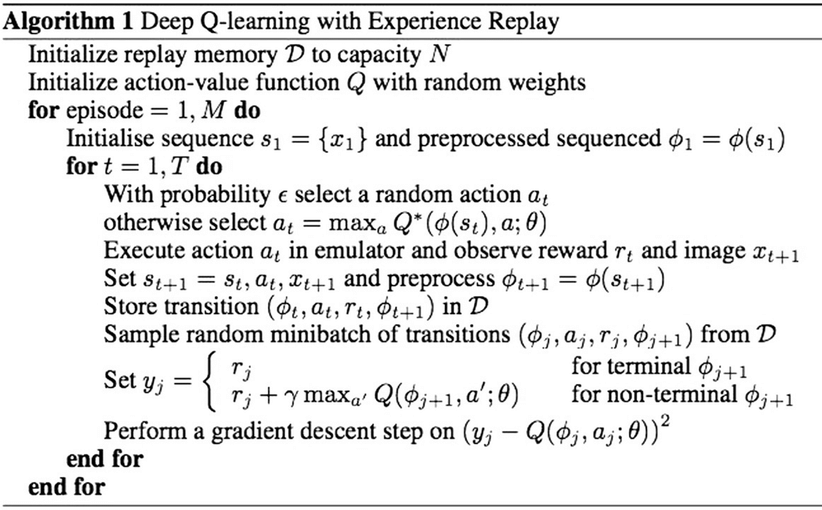
\includegraphics[scale=0.4]{gambar/dqn_algorithm.png}
    % Keterangan gambar yang diinputkan
    \caption{Algorithma \emph{Deep Q-Learning} \citep{deepQN}.}
    % Label referensi dari gambar yang diinputkan
    \label{fig:dqnAlgorithm}
\end{figure}

DQN memiliki kelemahan dimana perkiraan dari sebuah \emph{action value} nilainya terlalu besar.
DQN juga memiliki tendensi untuk mengejar \emph{action value} yang terbesar walau mungkin aksi tersebut tidaklah optimal pada situasi yang sedang dihadapi.
Melihat pada persamaan \ref{Eq:DQNEquation}, didapatkan $\max_{a'\in\mathcal{A}(s')}Q_*(s',a')$
yang mengambil nilai perkiraan maksimum secara implisit. Hal ini dapat menyebabkan \emph{maximization bias}
saat pembelajaran \cite{doubleQLearning}.

\emph{Double Deep Q-Learning} (DDQN) mencoba menstabilkan nilai \emph{action value} yang terlalu besar dengan menggunakan dua cabang \emph{hidden layer} pada DQN \citep{doubleDQN}.

\begin{figure}[H]
  \centering
    % Nama dari file gambar yang diinputkan
    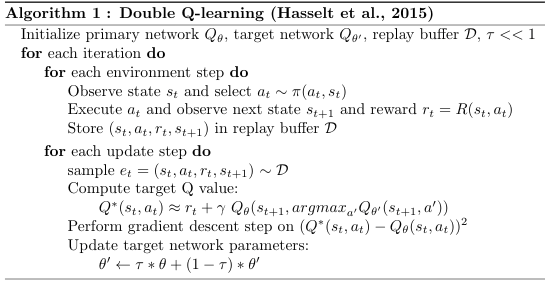
\includegraphics[scale=0.6]{gambar/ddqn_algorithm.png}
    % Keterangan gambar yang diinputkan
    \caption{Algoritma \emph{Double Deep Q-Learning} \citep{doubleDQN}.}
    % Label referensi dari gambar yang diinputkan
    \label{fig:ddqnAlgorithm}
\end{figure}

Algoritma DQN biasa melakukan \emph{uniform sampling} pada \emph{replay buffer} dimana
\emph{experience replay} diambil secara acak. Akan tetapi, hal ini dapat menyebabkan pengambilan sampel \emph{experience replay} yang kurang berguna pada saat pembelajaran.
Pada \emph{Prioritized Experience Replay} (PER), \emph{experience replay} yang lebih penting dalam
pembelajaran akan diambil lebih sering.
Prioritas ini didapatkan dengan mengithung nilai \emph{TD-error} \citep{prioritizedER}:

\begin{equation}
  \delta_{i} = r_{t} + \gamma \max_{a\in\mathcal{A}}Q_{\theta ^{-}}(s_{t+1},a) - Q_{\theta}(s_{t},a_{t})
  \label{Eq:DQNTDErrorEquation}
\end{equation}
atau pada \emph{Double} DQN:

\begin{equation}
  \delta_{i} = r_{t} + \gamma Q_{\theta^{-}} \left(s_{t+1}, \text{argmax}_{a\in\mathcal{A}}Q_{\theta ^{-}}(s_{t+1},a)\right) - Q_{\theta}(s_{t},a_{t}) 
  \label{Eq:DDQNTDErrorEquation}
\end{equation}

\begin{figure}[H]
  \centering
    % Nama dari file gambar yang diinputkan
    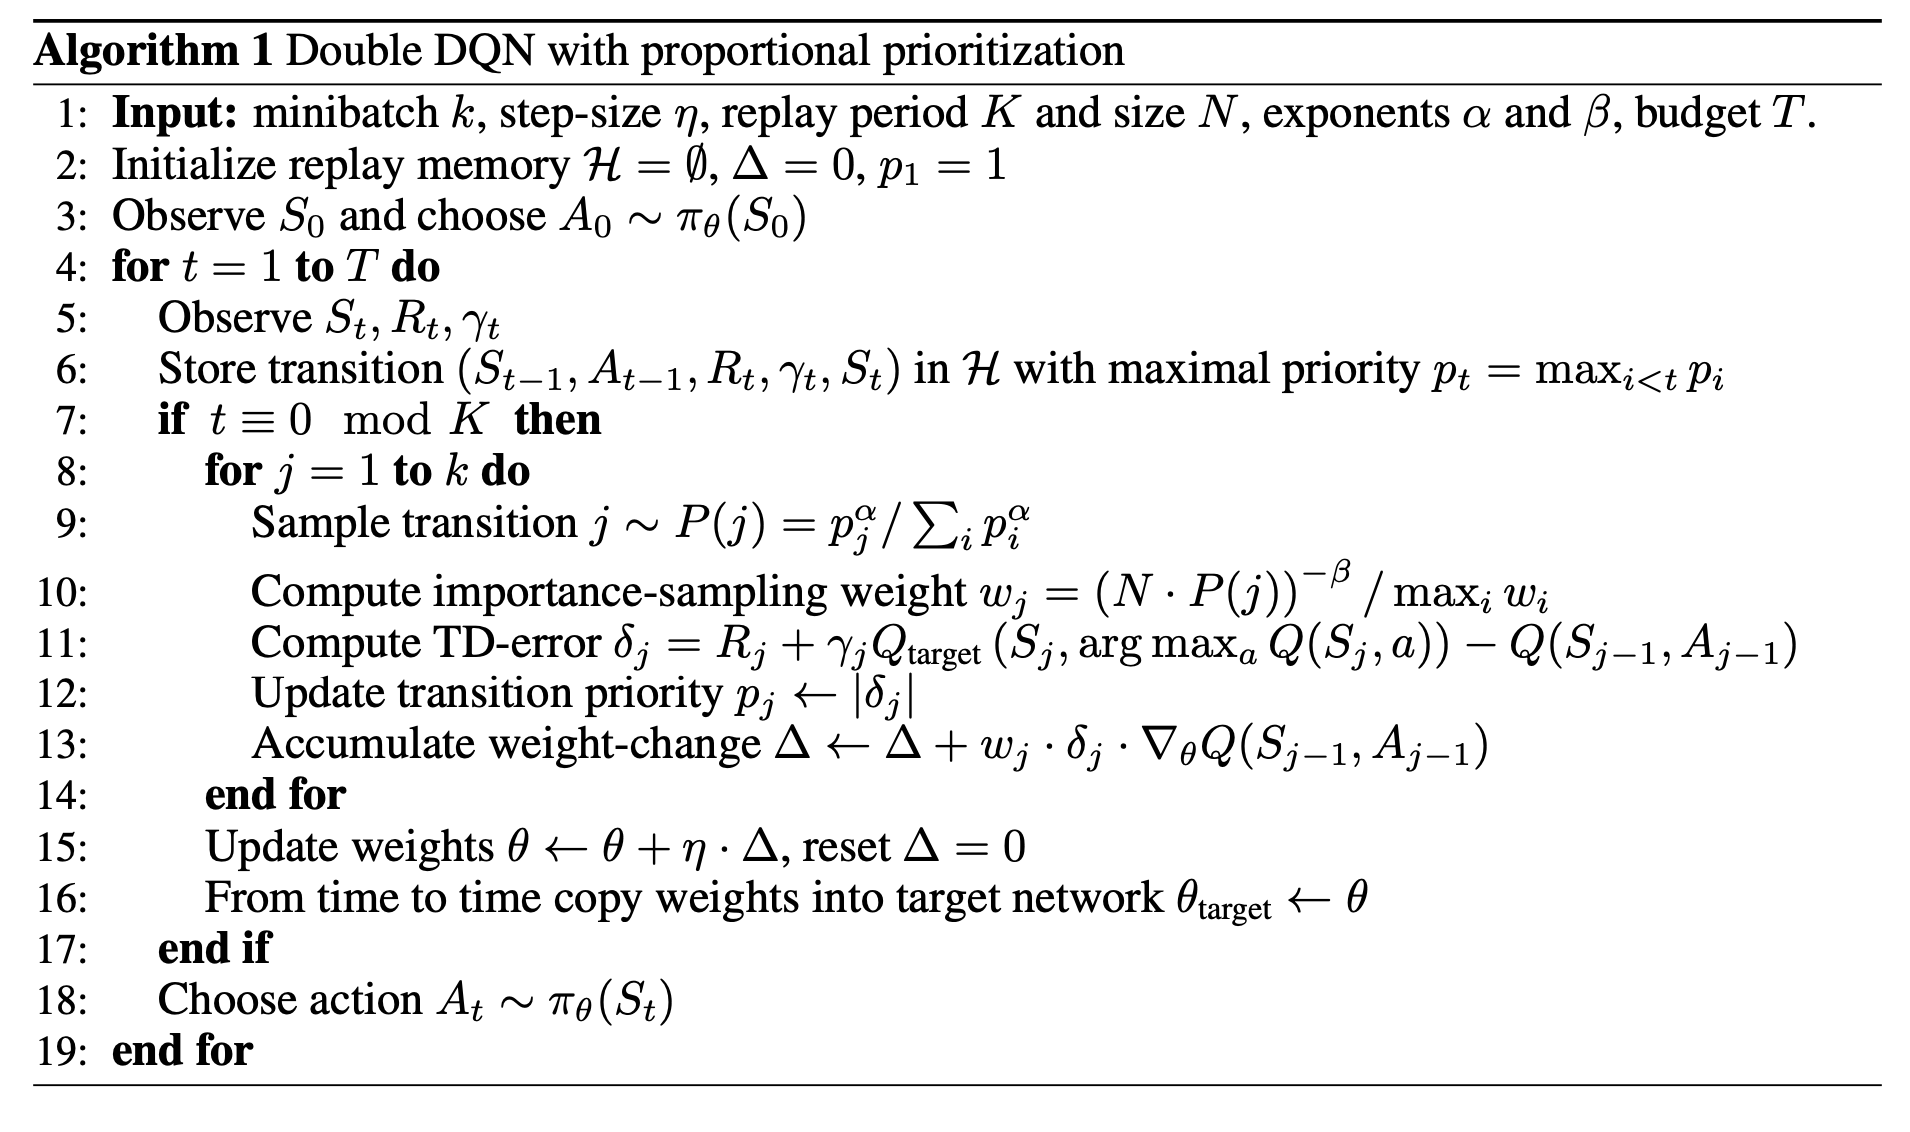
\includegraphics[scale=0.4]{gambar/ddqn_per_algorithm.png}
    % Keterangan gambar yang diinputkan
    \caption{Algorithma \emph{Double Deep Q-Learning} dengan \emph{Prioritized Experience Replay} \citep{prioritizedER}.}
    % Label referensi dari gambar yang diinputkan
    \label{fig:dqnPerAlgorithm}
\end{figure}

\emph{Dueling} DQN memisahkan neural network menjadi dua bagian, satu bagian mempelajari dan memberikan estimasi nilai pada seluruh \emph{timestep},
dan bagian lain menghitung nilai potensial (\emph{advantage}) dari sebuah aksi.
Kedua bagian ini digabungkan menjadi satu \emph{action-advantage Q function} \citep{duelingDQN}.

\begin{figure}[H]
  \centering
    % Nama dari file gambar yang diinputkan
    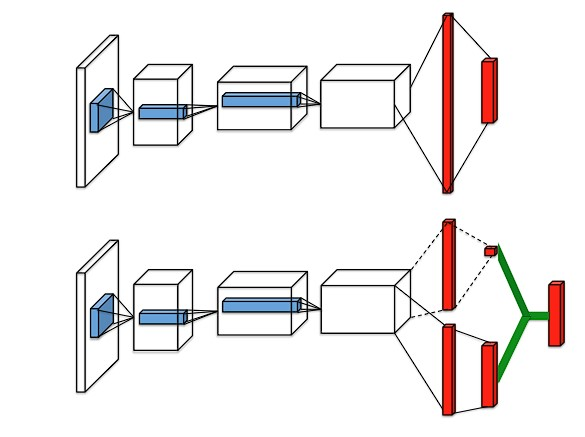
\includegraphics[scale=0.5]{gambar/dqn_vs_dueling_dqn_architecture.jpg}
    % Keterangan gambar yang diinputkan
    \caption{Arsitektur DQN (di atas) dibandingkan dengan Arsitektur \emph{Dueling} DQN (di bawah)}
    % Label referensi dari gambar yang diinputkan
    \label{fig:dqnVsDuelingDqnArchitecture}
\end{figure}

\section{Distributed Prioritized Experience Replay Deep Q-Networks (APE-X DQN)}

Distributed Prioritized Experience Replay Deep Q-Networks (Ape-X DQN) merupakan arsitektur DQN terdistribusi.
Dibandingkan dengan DQN biasanya, Ape-X DQN menggunakan banyak \emph{core} pada CPU sebagai \emph{actor} yang masing masing memiliki environment tersendiri.
\emph{Actor} tersebut akan mengumpulkan \emph{experience} yang didapatkan ke sebuah GPU \emph{learner}. 
\emph{Learner} tersebut akan mengambil sebuah sampel dengan metode \emph{prioritized experience} dan melakukan update pada \emph{neural network}. 
APE-X DQN ditemukan lebih efisien dan lebih baik daripada algoritma DQN lainnya dalam \emph{environment} game \emph{Atari} 2600 \citep{apexDQN}.

\begin{figure}[H]
  \centering
    % Nama dari file gambar yang diinputkan
    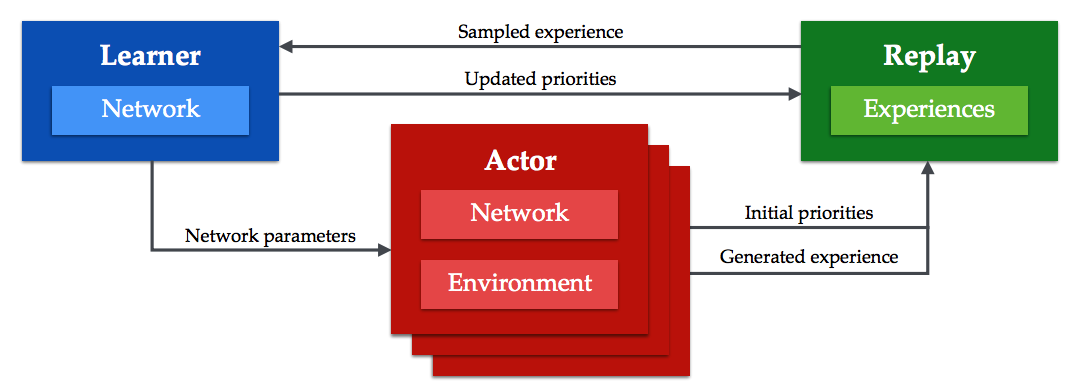
\includegraphics[scale=0.6]{gambar/apex1.png}
    % Keterangan gambar yang diinputkan
    \caption{Arsitektur APE-X dengan beberapa \emph{actor} dan menambahkan \emph{experiences} ke pada sebuah \emph{learner} \citep{apexDQN}.}
    % Label referensi dari gambar yang diinputkan
    \label{fig:apexDQNArchitecture}
\end{figure}

APE-X DQN memiliki seuah fungsi \emph{loss} untuk menghitung seluruh elemen dari \emph{batch} sebagai berikut:
\begin{equation}
  l_{t} (\theta) = \frac{1}{2}\left(G_{t}-q\left(S_{t},A_{t},\theta\right)\right)^2
\end{equation}
dengan 
\begin{equation}
  G_{t} = R_{t+1} + \gamma R_{t+2} + \dots + \gamma ^{n-1}R_{t+n} + \gamma ^{n}q\left(S_{t+n}, \text{argmax} q\left(S_{t+n},a,\theta \right)\theta ^{-}\right)
\end{equation}
dimana $t$ merupakan indeks dari \emph{experience} yang diambil dari \emph{replay} dimulai dari \emph{state} $S_{t}$ dan \emph{action} $A_{t}$,
dan $\theta^{-}$ menandakan parameter dari \emph{target network} \citep{apexDQN}.

\section{Proximal Policy Optimization}

\emph{Proximal Policy Optimization} (PPO) merupakan sebuah \emph{Policy Gradient Methods}. 
Berbeda dengan \emph{Q-Learning}, \emph{policy gradient methods} bekerja dengan cara menghitung sebuah estimator dari \emph{policy gradient} dan memasukannya ke
sebuah algoritma \emph{stochastic gradient ascent} \citep{ppo}. PPO mengoptimasi lebih lanjut dari mode \emph{Trust Region Policy Optimization} (TRPO).
Jika biasanya metode \emph{policy-gradient} melakukan satu \emph{gradient update} setiap sampel, PPO melakukan beberapa \emph{epochs} dari \emph{minibatch updates}. 
PPO memiliki beberapa keuntungan dari TRPO dengan implementasi yang lebih mudah, lebih baik dalam generalisasi, 
dan memiliki performa yang lebih baik dalam simulasi permainan game Atari dibandingkan dengan metode policy gradient yang lain.

PPO melakukan optimasi \emph{trust region} dengan mengganti batasan dari \emph{penalty} dalam sebuah fungsi \emph{objective}:
\begin{equation}
  L^{KLPEN} (\theta) = \mathbb{\hat{E}}\left[\frac{\pi_{\theta} (a_{t} | s_{t})}{\pi_{\theta_{old}} (a_{t} | s_{t})}\right] \hat{A}_{t} - \beta KL \left[\pi_{\theta_{old}}(. | s_{t}), \pi \theta(. | s_{t})\right]
\end{equation}
$\beta$ mengurangi \emph{objective} ketika sebuah \emph{policy} baru berbeda dengan \emph{policy} lama.
Jika \emph{KL-divergence} dari \emph{policy} baru dan lama lebih tinggi dari nilai target,
nilai $\beta$ akan dikurangi. Sebaliknya, jika nilai tersebut dibawah nilai target, maka nilai $\beta$ akan bertambah.

Pendekatan lain adalah menggunakan \emph{clipped surrogate objective}:
\begin{equation}
  L^{CLIP} (\theta) = \mathbb{\hat{E}}_{t}\left[\text{min}(r_{t}{\theta}\hat{A}_{t},\text{clip}(r_{t}(\theta),1-\epsilon,1+\epsilon)\hat{A}_{t})\right]
\end{equation}
dimana \emph{epsilon} adalah \emph{hyperparameter}. 
Saat rasio probabilitas dari \emph{policy} lama dan baru berada di luar ($1-\epsilon$) dan ($1+\epsilon$),
fungsi \emph{advantage} akan dipotong nilainya (\emph{clipped}). 
Dengan memotong nilai advantage, perubahan \emph{policy} yang diluar set \emph{hyperparameter} akan tidak sering terjadi, 
menjadikan proses \emph{update} lebih stabil.

\begin{figure}[H]
  \centering
    % Nama dari file gambar yang diinputkan
    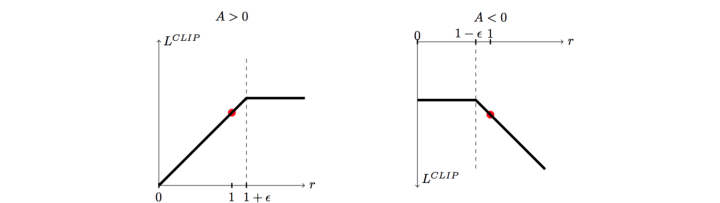
\includegraphics[scale=0.6]{gambar/ppo_clipped.png}
    % Keterangan gambar yang diinputkan
    \caption{Plot menunjugan sebuah timestep dari fungsi \emph{surrogate} $L^{CLIP}$
    sebagai fungsi rasio probabilitas. \emph{Advantage} positif (kiri) dan \emph{advantage} negatif (kanan).
    Lingkaran merah menunjukan titik awal untuk optimasi.}
    % Label referensi dari gambar yang diinputkan
    \label{fig:ppoClippedPlot}
\end{figure}

\section{Importance Weighted Actor-Learner Architecture (IMPALA)}

IMPALA merupakan sebuah \emph{framework} \emph{actor-critic} yang memisahkan antara acting dengan learning.
IMPALA menggunakan \emph{V-trace} dimana \emph{learner} mempelajari \emph{experience trajectory}.
GPU \emph{learner} pusat melakukan \emph{stochastic gradient descent} (SGD) pada sebuah \emph{tight loop} saat mengambil sampel 
\emph{batches} dari proses CPU \emph{actor} secara asinkronus \citep{impala}.

\emph{V-trace} merupakan sebuah algoritma RL \emph{off-policy actor-critic} yang mengurangi \emph{lag} dari \emph{actions} yang dibuat oleh \emph{actors}
dan saat \emph{learner} melakukan estimasi \emph{gradient}. 
Pada sebuah \emph{trajectory} $(x_{t}, a_{t}, r_{t})^{t=s+n}_{t=s}$ yang dibuat oleh \emph{actor} yang mengikut sebuah \emph{policy} $\mu$.
Target \emph{V-trace} pada \emph{$n$-steps} untuk $V(x_{s})$, dnegan nilai perkiraan pada \emph{state} $x_{s}$ di definisikan sebagai:
\begin{equation}
  v_{s} \stackrel{\text{def}}{=} V(x_{s}) + \sum^{s+n-1}_{t=s} \gamma^{t-s} \left(\Pi^{t-1}_{i=s}ci\right) \delta_{t}V
\end{equation}
dimana $\delta_{t}V \stackrel{\text{def}}{=} \rho_{t}\left(r_{t} + \gamma V(x_{t+1}) - V(x_{t})\right)$ merupakan perbedaan temporal untuk $V$,
dan $\rho_{t} \stackrel{\text{def}}{=} \text{min}\left(\overline{\rho}, \frac{\pi (a_{t}|x_{t})}{\mu (a_{t}|x_{t})}\right)$ dan 
$c_{i} \stackrel{\text{def}}{=} \text{min}\left(\overline{c}, \frac{\pi (a_{t}|x_{t})}{\mu (a_{t}|x_{t})}\right)$ adalah \emph{truncated importance sampling weight}.
Diasumsikan juga bahwa nilai \emph{truncation levels} adalah $\overline{\rho} \geq \overline{c}$ \citep{impala}.

Arsitektur IMPALA dapat mencapai \emph{throughput} yang tinggi, namun \emph{policy} yang digunakan untuk menghasilkan \emph{trajectory} terlambat selama beberapa \emph{update} jika dibandingkan dengan \emph{policy} yang ada pada \emph{learner} pada saat perhitungan gradien.
Oleh karena itu, IMPALA menggunakan \emph{V-trace off policy actor critic}

\begin{figure}[H]
  \centering
    % Nama dari file gambar yang diinputkan
    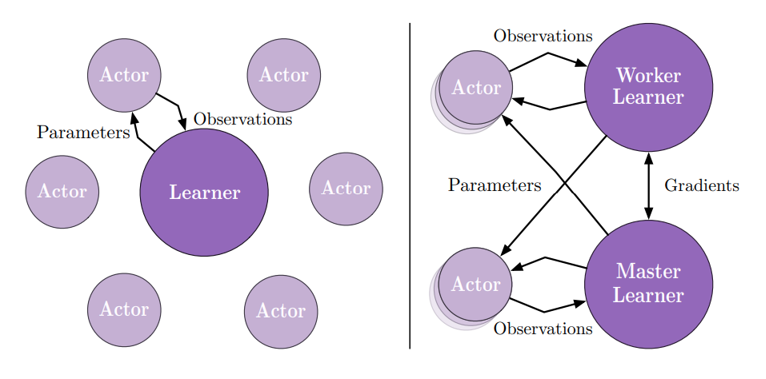
\includegraphics[scale=0.8]{gambar/impala_worker.png}
    % Keterangan gambar yang diinputkan
    \caption{Kiri: Sebuah learner. Setiap \emph{actor} menghasilkan \emph{trajectories} dan mengirimkannya melalui sebuah \emph{queue} kepada \emph{learner}.
    Sebelum memulai \emph{trajectory} selanjutnya, \emph{actor} menerima \emph{policy parameters} terbaru dari \emph{learner}.
    Kanan: Banyak \emph{learner}. \emph{Policy parameters} didistribusikan kepada lebih dari satu \emph{learner} yang bekerja secara sinkronus \citep{impala}.}
    % Label referensi dari gambar yang diinputkan
    \label{fig:impalaSingleVsMultipleLearner}
\end{figure}

\section{PettingZoo}

PettingZoo merupakan sebuah \emph{library} untuk membuat \emph{environment} yang mendukung \emph{multi agent reinforcement learning} (MARL).
PettingZoo menggunakan sebuah model formal \emph{game environment} baru yang disebut \emph{Agent Environment Cycle} (AEC). Dalam AEC, agen akan secara sekuensial melakukan \emph{observations}, mengambil \emph{actions}, mendapatkan \emph{rewards} yang diberikan dari agen lain, dan kemudian agen berikutnya melakukan \emph{actions}.
Model ini sangat cocok untuk game berbasis giliran \citep{pettingZoo}.

\begin{figure}[H]
  \centering
    % Nama dari file gambar yang diinputkan
    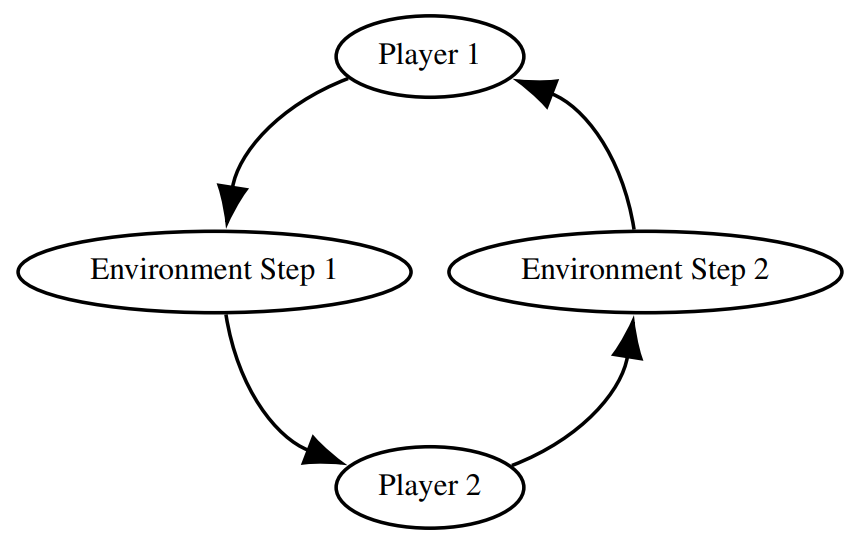
\includegraphics[scale=0.5]{gambar/actor_environment_cycle.png}
    % Keterangan gambar yang diinputkan
    \caption{Diagram AEC pada \emph{environment} dengan dua agen seperti catur}
    % Label referensi dari gambar yang diinputkan
    \label{fig:actorEnvironmentCycle}
\end{figure}

PettingZoo memiliki API yang mirip dengan Gym. Kemiripan API ini memudahkan pengguna untuk menggunakan ataupun mengubah \emph{library environment} dari Gym ke PettingZoo ataupun sebaliknya.

% Contoh pembuatan potongan kode
\begin{lstlisting}[
  language=Python,
  caption={Contoh dasar penggunaan API Gym.},
  label={lst:gymAPI}
]
  import gym
  env = gym.make('CartPole-v0')
  observation = env.reset()
  for _ in range(1000):
  action = policy(observation)
  observation, reward, done, info = env.step(action)
\end{lstlisting}

\begin{lstlisting}[
  language=Python,
  caption={Contoh dasar penggunaan API PettingZoo.},
  label={lst:pettingZooAPI}
]
  from ray.rllib.examples.env.multi_agent
  import MultiAgentCartPole
  env = MultiAgentCartPole()
  observation = env.reset()
  for _ in range(1000):
  actions = policies(agents, observation)
  observation, rewards, dones,
  infos = env.step(actions)
\end{lstlisting}

\section{RLlib}
RLlib adalah sebuah \emph{library} RL yang merupakan bagian dari \emph{open source Ray project} yang menawarkan
algoritma RL berskala dan performa tinggi untuk komputasi terdistribusi \citep{rllib}.
RLlib menawarkan beberapa koleksi dan referensi algoritma dan juga abstraksi \emph{scalable} untuk memudahkan
pembuatan algoritma baru. RLlib mendukung beberapa \emph{library} \emph{environment} seperti \emph{OpenAI Gym},
\emph{PettingZoo}, dan juga simulator eksternal seperti \emph{Unity3D} atau \emph{game engine} lainnya.
  \cleardoublepage

  % Bab 3 desain dan implementasi
  \chapter{METODOLOGI}
% Ubah bagian-bagian berikut dengan isi dari desain dan implementasi

Eksperimen pada penelitian ini akan mengikuti konvensi standar eksperimen DRL sebelumnya, yaitu menguji coba dan mengevaluasi performa agen dalam \emph{environment} dengan membandingkan nilai \emph{reward} yang diterima oleh agen.
Agen akan melakukan \emph{training} dalam \emph{environment} yang telah dibuat.

\section{Perangkat}

Eksperimen dalam penelitian ini menggunakan beberapa perangkat keras dan perangkat lunak.


\subsection{Perangkat Keras}

Proses \emph{training} agen dilakukan dengan sebuah komputer. Komputer tersebut memiliki spesifikasi:
\begin{itemize}
  \item Processor: Intel I7 9700K
  \item Graphics Card: RTX 2080 SUPER
  \item RAM: 32GB DDR4
  \item SSD: 512GB NVME PCIE Gen 3
\end{itemize}

\subsection{Perangkat Lunak}

Beberapa pernagkat lunak digunakan untuk menunjang pembuatan \emph{environment} dan agen DRL dalam eksperimen ini:
\begin{itemize}
  \item Python
  \item Visual Studio Code
  \item Tensorboard
  \item Ray RLlib
  \item Pygame
  \item PettingZoo
  \item Numpy
  \item Matplotlib
\end{itemize}
\section{Desain Environment}
Desain dari \emph{environment} adalah modifikasi dari Inquisitive Otter's Civ6 environment \citep{civ6Environment}. 
Desain awal dari \emph{environment} ini hanya memiliki sebuah agen \emph{attacker} dan memiliki mekanisme yang kurang sesuai dengan mekanisme Civ6.
\emph{Environment} yang sudah dimodifikasi ini juga sudah diimplementasikan ke dalam PettingZoo.
Implementasi ke PettingZoo memudahkan untuk mengintegrasikan \emph{environment} ini dengan library RL lain.

\subsection{Area dan Posisi}
\emph{Environment} merupakan area \emph{pointy top hexagonal grid} berukuran 8x8. Di tengah area tersebut terdapat sebuah kota.
\emph{Environment} yang sudah termodifikasi memiliki dua jenis agen yaitu agen \emph{attacker} dan agen \emph{defender}.
Agen \emph{attacker} memiliki 3 \emph{unit} jarak dekat (\emph{melee}) (\emph{warrior}) dan 2 \emph{unit} jarak jauh (\emph{ranged}) (\emph{slinger}).
Agen \emph{defender} memiliki 2 \emph{warrior} dan 1 \emph{slinger}.

Penempatan \emph{unit} agen dilakukan secara acak dengan pembatasan.
\emph{Unit} agen \emph{attacker} ditempatkan minimal sejauh 5 lantai dari kota di tengah area.
\emph{Unit} agen \emph{defender} berada di lantai sebelah kota.


\begin{figure}[H]
  \centering
    % Nama dari file gambar yang diinputkan
    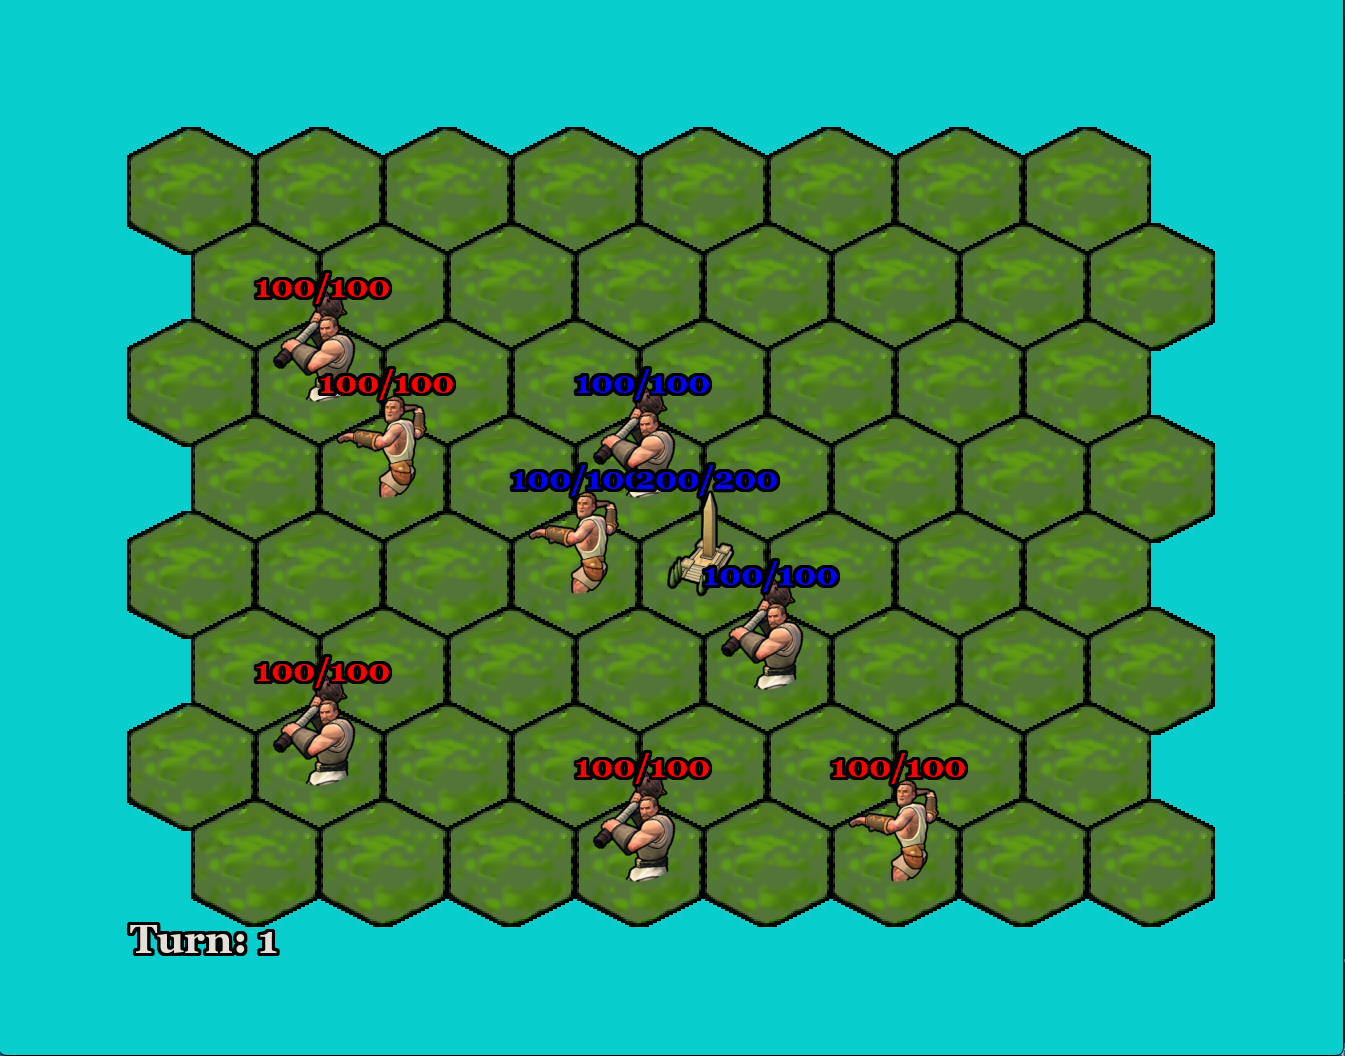
\includegraphics[scale=0.3]{gambar/environment_screenshot.png}
    % Keterangan gambar yang diinputkan
    \caption{\emph{Screenshot environment} dalam mode \emph{render}. \emph{Unit} milik agen \emph{attacker} memiliki teks \emph{hit points} berwarna merah dan unit milik agen \emph{defender} memiliki teks \emph{hit points} berwarna biru.}
    % Label referensi dari gambar yang diinputkan
    \label{fig:environmentScreenshot}
\end{figure}

\subsection{Unit dan Kota}
\emph{Unit} yang paling banyak jumlahnya dalam \emph{environment} ini adalah \emph{warrior}. 
\emph{Warrior} merupakan \emph{melee unit}, yang mana hanya dapat menyerang lawan yang berada di sebelah unit tersebut.
\emph{Warrior} memiliki attribut sebagai berikut:
\begin{itemize}
  \item HP: 100
  \item \emph{Movement Points}: 2
  \item \emph{Combat Strength}: 20
\end{itemize}

Jenis \emph{Unit} kedua adalah \emph{slinger}. \emph{Slinger} merupakan \emph{ranged unit} yang memiliki jarak sejauh 1 lantai.
\emph{Slinger} dapat menyerang \emph{unit} lain yang berdekatan dengan \emph{slinger} tanpa menerima \emph{damage} balasan dari \emph{unit} yang diserang.
\emph{Slinger} memiliki attribut sebagai berikut:
\begin{itemize}
  \item HP: 100
  \item \emph{Movement Points}: 2
  \item \emph{Combat Strength}: 5
  \item \emph{Ranged Strength}: 15
\end{itemize}

Kota merupakan tujuan utama yang perlu dihancurkan oleh agen \emph{attacker}. 
Kota akan berusaha melakukan perbaikan pada gilirannya dengan menambahkan +20 HP jika HP yang dimilikinya kurang dari nilai maksimum.
Kota tidak dapat melakukan perbaikan jika terdapat minimal tiga \emph{melee unit} milik agen \emph{attacker}.
Berikut adalah attribut dari kota:
\begin{itemize}
  \item HP: 200
  \item \emph{Combat Strength}: 28
\end{itemize}

\begin{figure}[!htb]
  \begin{minipage}{0.32\textwidth}
    \centering
    
\includegraphics[width=\linewidth]{gambar/warrior_1.png}
    \caption{\emph{Unit warrior}}\label{Fig:warrior}
  \end{minipage}\hfill
  \begin{minipage}{0.32\textwidth}
    \centering
    
\includegraphics[width=\linewidth]{gambar/slinger_1.png}
    \caption{\emph{Unit slinger}}\label{Fig:slinger}
  \end{minipage}
  \begin{minipage}{0.32\textwidth}
    \centering
    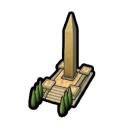
\includegraphics[width=\linewidth]{gambar/city.png}
    \caption{Kota}\label{Fig:kota}
  \end{minipage}
\end{figure}

\subsection{Giliran dan Pergerakan Unit Agen}
Agen dapat mengkontrol \emph{unit} mereka pada giliran yang sudah ditentukan. 
\emph{Environment} dimulai dengan giliran agen \emph{attacker}, dilanjutkan oleh giliran kota, dan kemudian
ke giliran agen \emph{defender} sebelum kembali ke agen \emph{attacker}. 
Pergerakan dan pemilihan unit oleh agen dilakukan secara sekuensial. Pertama, agen akan memilih unit pertama mereka.
Agen akan melakukan pergerakan dengan unit yang telah dipilih sampai unit tersebut tidak lagi memiliki \emph{movement points}
pada giliran tersebut.
Setelah itu, agen akan berpindah ke unit selanjutnya. Hal ini akan berulang sampai agen tidak lagi memiliki unit yang masih
mempunyai \emph{movement points}. Jika agen sudah tidak memiliki unit yang masih mempunyai \emph{movement points}
maka agen akan mengakhiri giliran mereka dan giliran berikutnya akan dimulai. 
Sebuah \emph{episode} dari \emph{environment} akan berakhir ketika 20 giliran sudah berlalu, kota sudah hancur, atau seluruh \emph{unit}
milik agen \emph{attacker} mati.
Berikut flowchart dari pergerakan dan pemilihan sekuensial ini:

\begin{figure}[H]
  \centering
    % Nama dari file gambar yang diinputkan
    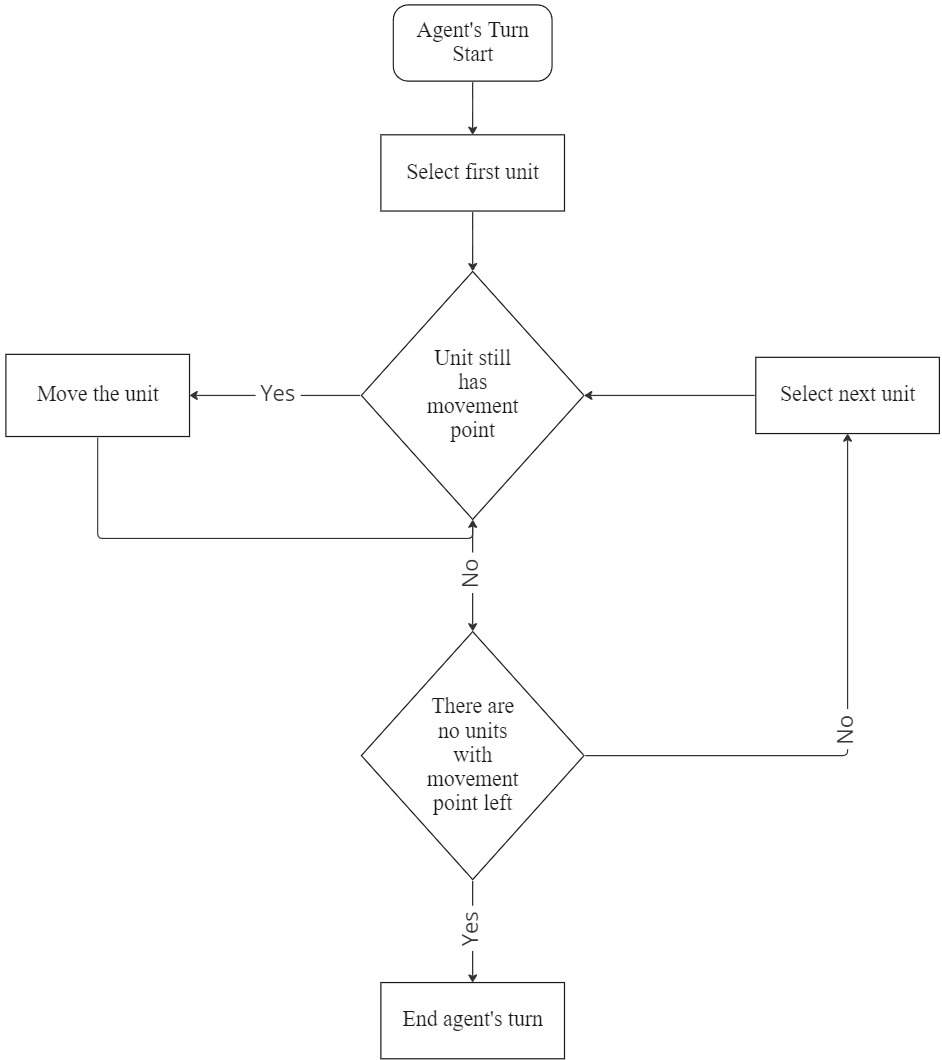
\includegraphics[scale=0.48]{gambar/unit_sequential_movement.jpg}
    % Keterangan gambar yang diinputkan
    \caption{\emph{Flowchart} pergerakan dan pemilihan sekuensial unit agen}
    % Label referensi dari gambar yang diinputkan
    \label{fig:sequentialMovementFlowchart}
\end{figure}

\subsection{Action Space}
\emph{Action space} merupakan kemungkinan yang dapat diambil oleh agen untuk melakukan sebuah \emph{action}.
\emph{Action space} yang digunakan dalam \emph{environment} ini adalah berupa 7 \emph{discrete actions}.
7 \emph{discrete actions} tersebut merupakan 6 sisi dimana unit dapat bergerak ke dan 1 \emph{action} unit tidak bergerak ke manapun.

% input gambar
\begin{figure}[H]
  \centering
    % Nama dari file gambar yang diinputkan
    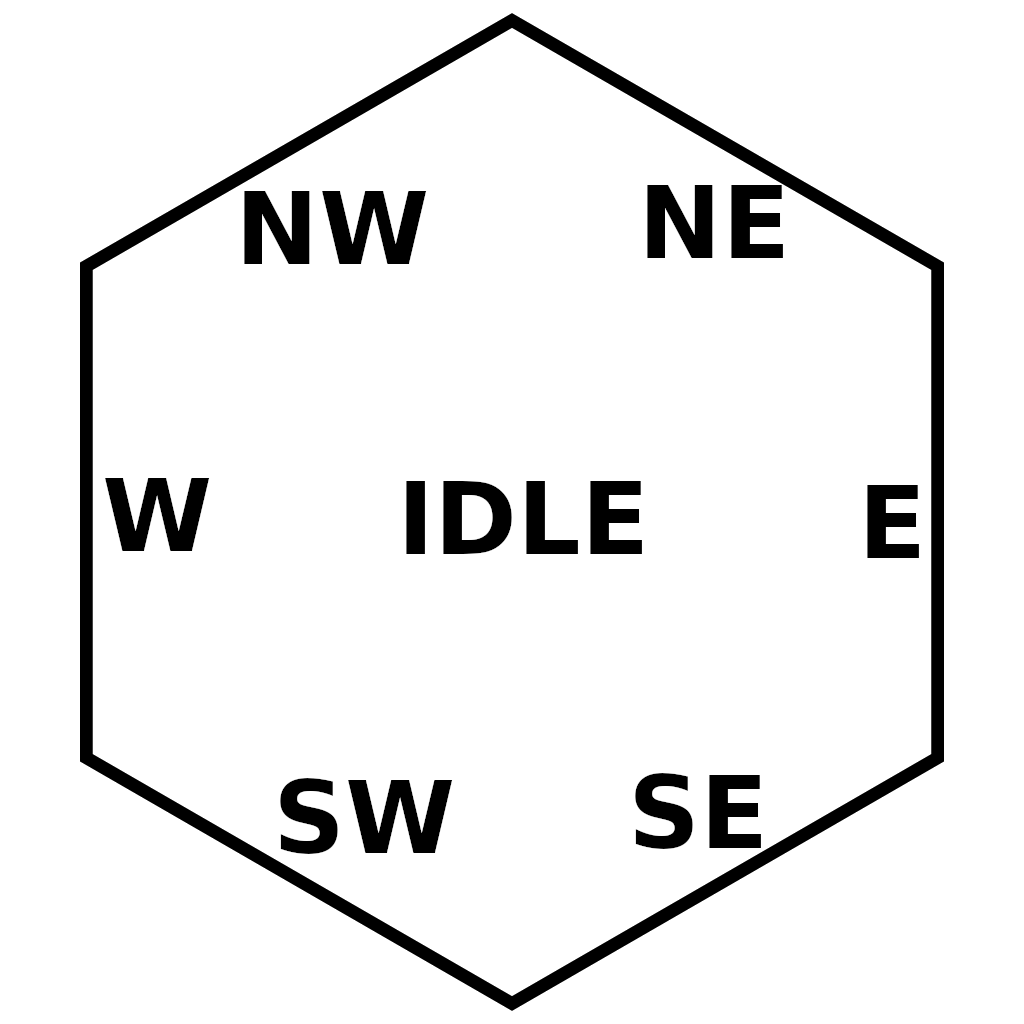
\includegraphics[scale=0.6]{gambar/hex_action.png}
    % Keterangan gambar yang diinputkan
    \caption{7 \emph{actions} yang dapat diambil oleh AI dalam \emph{Hexagonal tile}}
    % Label referensi dari gambar yang diinputkan
    \label{fig:hex_action}
\end{figure}

\subsection{Observation Space}
\emph{Observation Space} merupakan kumpulan \emph{state} dalam \emph{environment} yang didapatkan oleh agen saat melakukan observasi.
Agen dalam \emph{environment} penelitian ini melakukan \emph{complete observation}. 
Kedua agen mendapatkan informasi \emph{state} yang penuh dan sama saat melakukan observasi.
Seluruh nilai \emph{state} dinormalisasi sehingga nilainya berupa 0 sampai 1.
Berikut merupakan \emph{state} yang didapatkan oleh agen saat observasi:
\begin{itemize}
  \item Jarak seluruh unit dari kota: $x_{1}, y_{1}, \dots x_{n}, y_{n}$
  \item Nilai HP dari seluruh unit: $HP_{1}, \dots HP_{n}$
  \item Nilai movement points dari seluruh unit: $MP_{1}, \dots MP_{n}$
\end{itemize}

\subsection{Reward Agen}
\emph{Reward} merupakan nilai yang diberikan kepada agen ketika agen tersebut melakukan sebuah \emph{action}.
Karena \emph{environment} pada penelitian ini merupakan \emph{asymmetric}, maka terdapat dua tipe \emph{reward}:
\emph{general rewards} dan \emph{attacker rewards}. 
\emph{General rewards} adalah tipe \emph{reward} yang diberikan ke agen \emph{attacker} dan \emph{defender}.
Sedangkan \emph{attacker rewards} hanya diberikan pada agen \emph{attacker}.
Berikut \emph{reward} tersebut:
\begin{itemize}
  \item General rewards: \begin{itemize}
      \item Bergerak ke luar batas \emph{environment} = -1
      \item Melakukan \emph{healing} pada sebuah \emph{unit} = +0.1
      \item Menyerang \emph{unit} lawan = +0.2
      \item Mematikan \emph{unit} lawan = +3
  \end{itemize}
  \item Attacker rewards: \begin{itemize}
      \item Menghancurkan kota = +20
      \item Menyerang kota = +0.5
      \item Kota melakukan perbaikan = -0.3
      \item Sebuah \emph{unit} mati = -1
      \item Sebuah giliran telah berlalu = -1
  \end{itemize}
\end{itemize}

Agen \emph{attacker} akan mendapatkan +20 poin ketika menghancurkan kota, karena itu merupakan tujuan utama dari agen \emph{attacker}.
Jika sebuah \emph{unit} agen \emph{attacker} mati atau sebuah giliran telah berlalu maka agen \emph{attacker} akan mendapatkan -1 point
Hal ini untuk memaksa agen \emph{attacker} agar menyelesaikan tujuannya secepat mungkin dan meminimalisir kehilangan \emph{unit}.

Agen \emph{defender} yang memiliki tujuan untuk mencoba mencegah agen \emph{attacker} mendapatkan +3 poin ketika sebuah \emph{unit}
agen \emph{attacker} mati. Tidak diberikan penalti pada agen \emph{defender} ketika unit mereka mati karena pada eksperimen sebelumnya,
hal tersebut membuat agen \emph{defender} terlalu pasif. Kedua agen akan mendapatkan penalti ketika mencoba untuk menggerakan \emph{unit}
milik mereka keluar dari batas \emph{environment}.

\section{Implementasi Algoritma DRL}
Implementasi algoritma dalam penelitian ini menggunakan RLlib versi 2.0.0.
Kami menggunakan RLlib dengan alasan bahwa algoritma yang diimplementasikan dalam \emph{library} ini
sudah diverifikasi oleh berbagai pihak, sehingga menghindari adanya \emph{bug} pada implementasi manual.
Alasan kedua adalah kemampuan RLlib untuk diintegrasikan dengan simulator eksternal seperti Unity3D
dan \emph{game engine} lainnya \citep{rllibDocumentation}.
Mengingat bahwa manfaat dari penelitian ini adalah memberi contoh implementasi DRL
bagi \emph{game developer}.
Reproduksi akan hasil eksperimen dari penelitian juga akan dipermudah dengan 
menggunakan sebuah \emph{open source library} RL seperti RLlib.
Terdapat 4 algoritma SOTA DRL yang diimplementasikan dalam \emph{environment} dalam
eksperimen penelitian ini: DQN, APE-X DQN, PPO, IMPALA. 
Algoritma-algoritma tersebut dipilih karena mencakup beberapa bidang dari DRL seperti
on-policy, off-policy, dan distributed learning.
\emph{Hyperparameter} dari algoritma-algoritma tersebut mengikuti \emph{hyperparameter}
dasar yang diberikan secara \emph{default} oleh RLlib 2.0.0 dengan beberapa pengecualian:
\begin{itemize}
  \item num\_rollout\_workers: Mengatur akan jumlah instansi parallel training yang berjalan.
  angka 3 dipilih karena APE-X DQN menggunakan 2 CPU core setiap pada \emph{rollout\_workers}
  dan 2 core dasar. Dengan 3 \emph{rollout\_workers}, APE-X menggunakan seluruh 8 core dari i7 9700K
  secara penuh.

  \item multi\_agent: untuk membedakan \emph{policy}
  yang digunakan oleh agen \emph{attacker} dan \emph{defender}

  \item num\_env\_steps\_sampled: jumlah \emph{environment steps} yang dilakukan sebelum training selesai.
  Dipilih angka 10 juta karena jika melampaui angka ini, APE-X DQN akan menghabiskan lebih dari 32GB RAM.
  Kapasitas RAM yang terdapat pada spesifikasi hanya 32GB.
  
  \item num\_gpus: Digunakan satu GPU dalam training.
\end{itemize}

\begin{lstlisting}[
  language=Python,
  caption={Cuplikan kode setting config (hyperparameter)},
  label={lst:customHyperparameter}
]
config.multi_agent(

  policies={pid: (None, obs_space, act_space, {}) for pid in

            test_env.env.agents},

  policy_mapping_fn=(lambda agent_id, episode, **kwargs: agent_id),

  )  

config.num_gpus = 1
config.rollouts(num_rollout_workers=3)
    
\end{lstlisting}

Selain \emph{hyperparameter} yang sama (\emph{common-configs}), setiap algoritma memiliki \emph{hyperparameter}
tersendiri yang khusus untuk algoritma tersebut (\emph{specific-configs}).

\subsection{Implementasi DQN}
DQN yang digunakan dalam implementasi RLlib secara default adalah \emph{Double Dueling} DQN
dengan PER.

\begin{figure}[H]
  \centering
    % Nama dari file gambar yang diinputkan
    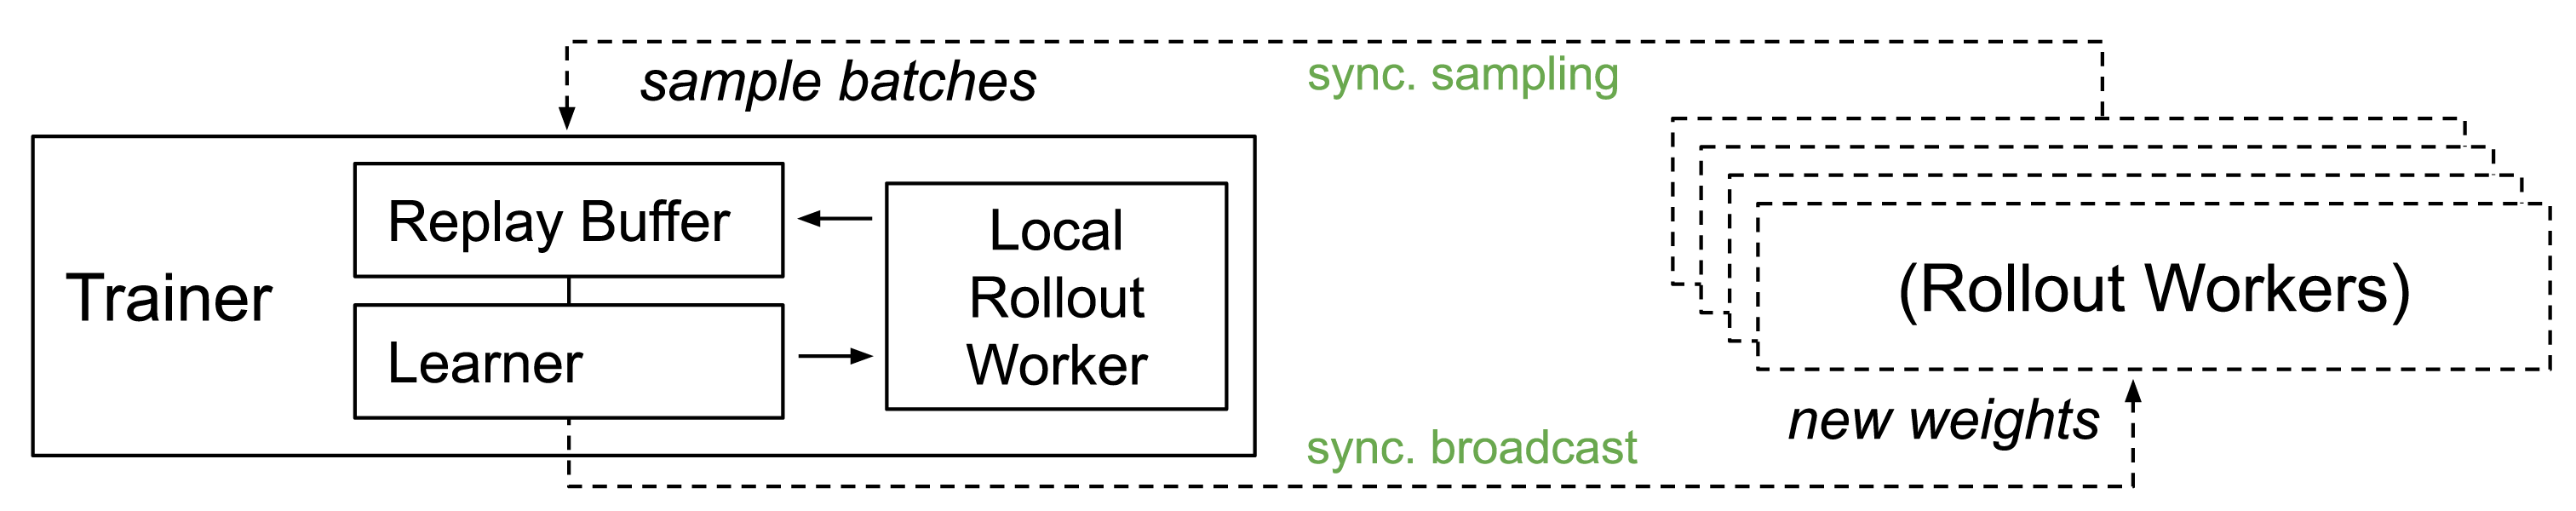
\includegraphics[scale=0.6]{gambar/rllib_dqn_architecture.png}
    % Keterangan gambar yang diinputkan
    \caption{Arsitektur DQN pada RLlib 2.0.0 \citep{rllibDocumentation}}
    % Label referensi dari gambar yang diinputkan
    \label{fig:rllib_dqn_architecture}
\end{figure}

\begin{lstlisting}[
  language=Python,
  caption={DQN-specific configs},
  label={lst:dqnSpecificConfigs}
]
self.num_atoms = 1
self.v_min = -10.0
self.v_max = 10.0
self.noisy = False
self.sigma0 = 0.5
self.dueling = True
self.hiddens = [256]
self.double_q = True
self.n_step = 1
self.before_learn_on_batch = None
self.training_intensity = None
self.td_error_loss_fn = "huber"
self.categorical_distribution_temperature = 1.0

# Changes to SimpleQConfig's default:
self.replay_buffer_config = {
    "type": "MultiAgentPrioritizedReplayBuffer",
    # Specify prioritized replay by supplying a buffer type that supports
    # prioritization, for example: MultiAgentPrioritizedReplayBuffer.
    "prioritized_replay": DEPRECATED_VALUE,
    # Size of the replay buffer. Note that if async_updates is set,
    # then each worker will have a replay buffer of this size.
    "capacity": 50000,
    "prioritized_replay_alpha": 0.6,
    # Beta parameter for sampling from prioritized replay buffer.
    "prioritized_replay_beta": 0.4,
    # Epsilon to add to the TD errors when updating priorities.
    "prioritized_replay_eps": 1e-6,
    # The number of continuous environment steps to replay at once. This may
    # be set to greater than 1 to support recurrent models.
    "replay_sequence_length": 1,
    # Whether to compute priorities on workers.
    "worker_side_prioritization": False,
}
# fmt: on
\end{lstlisting}

\subsection{Implementasi APE-X DQN}
Implementasi APE-X DQN dalam RLlib 2.0.0 menggunakan implementasi DQN yang ada dengan
tambahan \emph{distributed prioritezed experience replay} (APE-X) untuk skalabilitas
yang mencapai ratusan CPU dengan satu GPU \emph{learner}. Pada \emph{specific-configs}
yang digunakan oleh APE-X DQN, digunakan 32 \emph{rollout\_workers}. Setting \emph{rollout\_workers}
tersebut terganti oleh 3 \emph{rollout\_workers} yang dideklarasikan pada \ref{lst:customHyperparameter}.

\begin{figure}[H]
  \centering
    % Nama dari file gambar yang diinputkan
    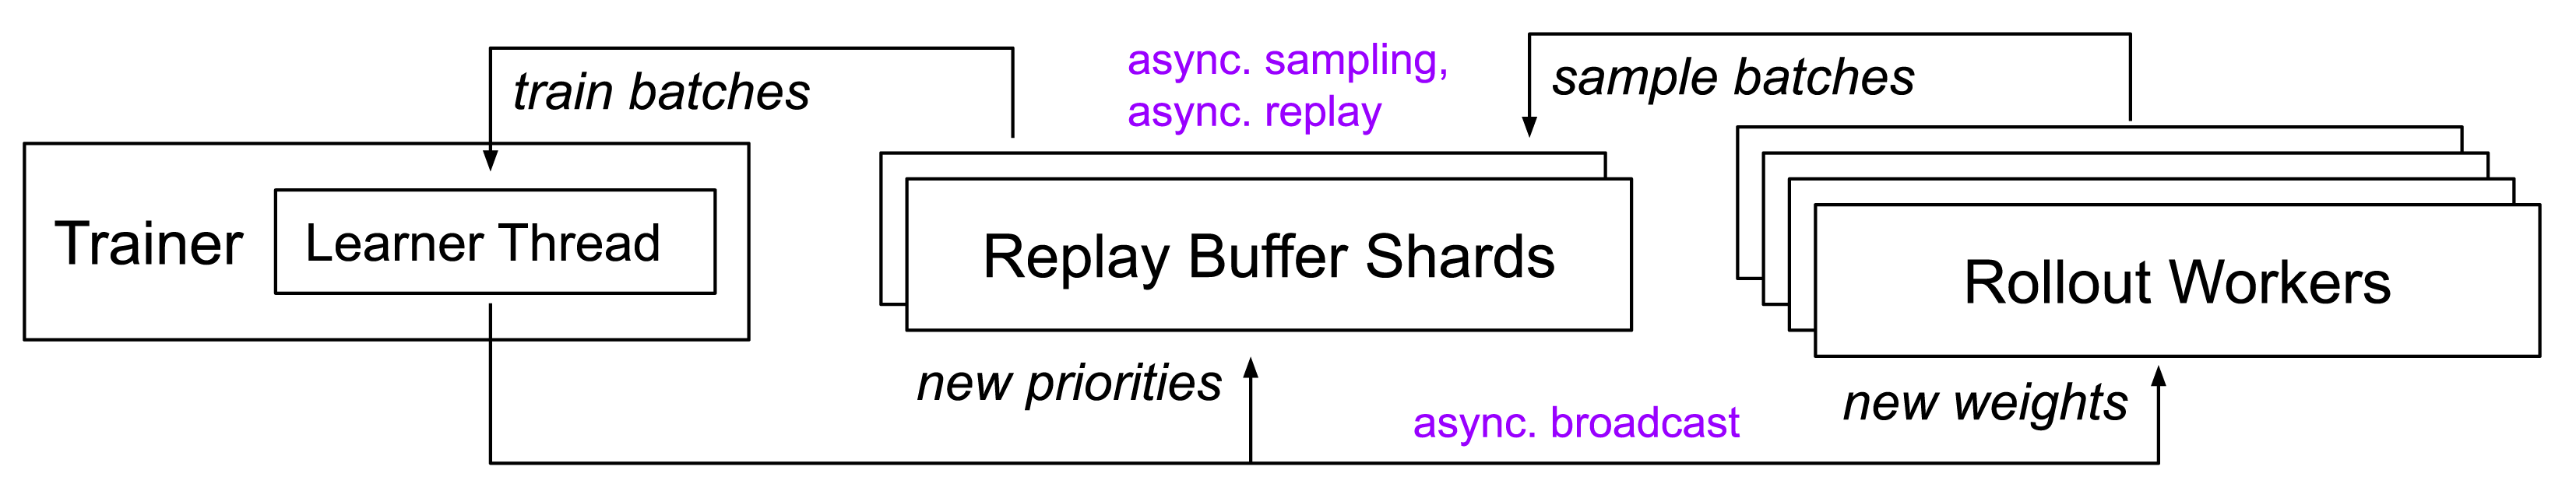
\includegraphics[scale=0.6]{gambar/rllib_apex-dqn_architecture.png}
    % Keterangan gambar yang diinputkan
    \caption{Arsitektur APE-X DQN pada RLlib 2.0.0 \citep{rllibDocumentation}}
    % Label referensi dari gambar yang diinputkan
    \label{fig:rllib_apex-dqn_architecture}
\end{figure}

\begin{lstlisting}[
  language=Python,
  caption={Cuplikan kode setting config (hyperparameter)},
  label={lst:apexDqnSpecificConfigs}
]
# APEX-DQN settings overriding DQN ones:
# .training()
self.optimizer = merge_dicts(
    DQNConfig().optimizer, {
        "max_weight_sync_delay": 400,
        "num_replay_buffer_shards": 4,
        "debug": False
    })
self.n_step = 3
self.train_batch_size = 512
self.target_network_update_freq = 500000
self.training_intensity = 1
# Number of timesteps to collect from rollout workers before we start
# sampling from replay buffers for learning. Whether we count this in agent
# steps  or environment steps depends on config["multiagent"]["count_steps_by"].
self.num_steps_sampled_before_learning_starts = 50000

# max number of inflight requests to each sampling worker
# see the AsyncRequestsManager class for more details
# Tuning these values is important when running experimens with large sample
# batches. If the sample batches are large in size, then there is the risk that
# the object store may fill up, causing the store to spill objects to disk.
# This can cause any asynchronous requests to become very slow, making your
# experiment run slowly. You can inspect the object store during your
# experiment via a call to ray memory on your headnode, and by using the ray
# dashboard. If you're seeing that the object store is filling up, turn down
# the number of remote requests in flight, or enable compression in your
# experiment of timesteps.
self.max_requests_in_flight_per_sampler_worker = 2
self.max_requests_in_flight_per_replay_worker = float("inf")
self.timeout_s_sampler_manager = 0.0
self.timeout_s_replay_manager = 0.0
# APEX-DQN is using a distributed (non local) replay buffer.
self.replay_buffer_config = {
    "no_local_replay_buffer": True,
    # Specify prioritized replay by supplying a buffer type that supports
    # prioritization
    "type": "MultiAgentPrioritizedReplayBuffer",
    "capacity": 2000000,
    # Alpha parameter for prioritized replay buffer.
    "prioritized_replay_alpha": 0.6,
    # Beta parameter for sampling from prioritized replay buffer.
    "prioritized_replay_beta": 0.4,
    # Epsilon to add to the TD errors when updating priorities.
    "prioritized_replay_eps": 1e-6,
    # Whether all shards of the replay buffer must be co-located
    # with the learner process (running the execution plan).
    # This is preferred b/c the learner process should have quick
    # access to the data from the buffer shards, avoiding network
    # traffic each time samples from the buffer(s) are drawn.
    # Set this to False for relaxing this constraint and allowing
    # replay shards to be created on node(s) other than the one
    # on which the learner is located.
    "replay_buffer_shards_colocated_with_driver": True,
    "worker_side_prioritization": True,
    # Deprecated key.
    "prioritized_replay": DEPRECATED_VALUE,
}

# .rollouts()
self.num_workers = 32
self.rollout_fragment_length = 50
self.exploration_config = {
    "type": "PerWorkerEpsilonGreedy",
}

# .resources()
self.num_gpus = 1

# .reporting()
self.min_time_s_per_iteration = 30
self.min_sample_timesteps_per_iteration = 25000

# fmt: on
\end{lstlisting}

\subsection{Implementasi PPO}
Implementasi PPO dari RLlib 2.0.0 menggunakan \emph{clipped objective} dan \emph{KL-penalty}.
Multi-GPU \emph{optimizer} RLlib meletakkan data di GPU memori untuk menghindari transfer yang tidak diperlukan
dari \emph{host memory}, sehingga performa lebih baik dari implementasi secara \emph{naive}.

\begin{figure}[H]
  \centering
    % Nama dari file gambar yang diinputkan
    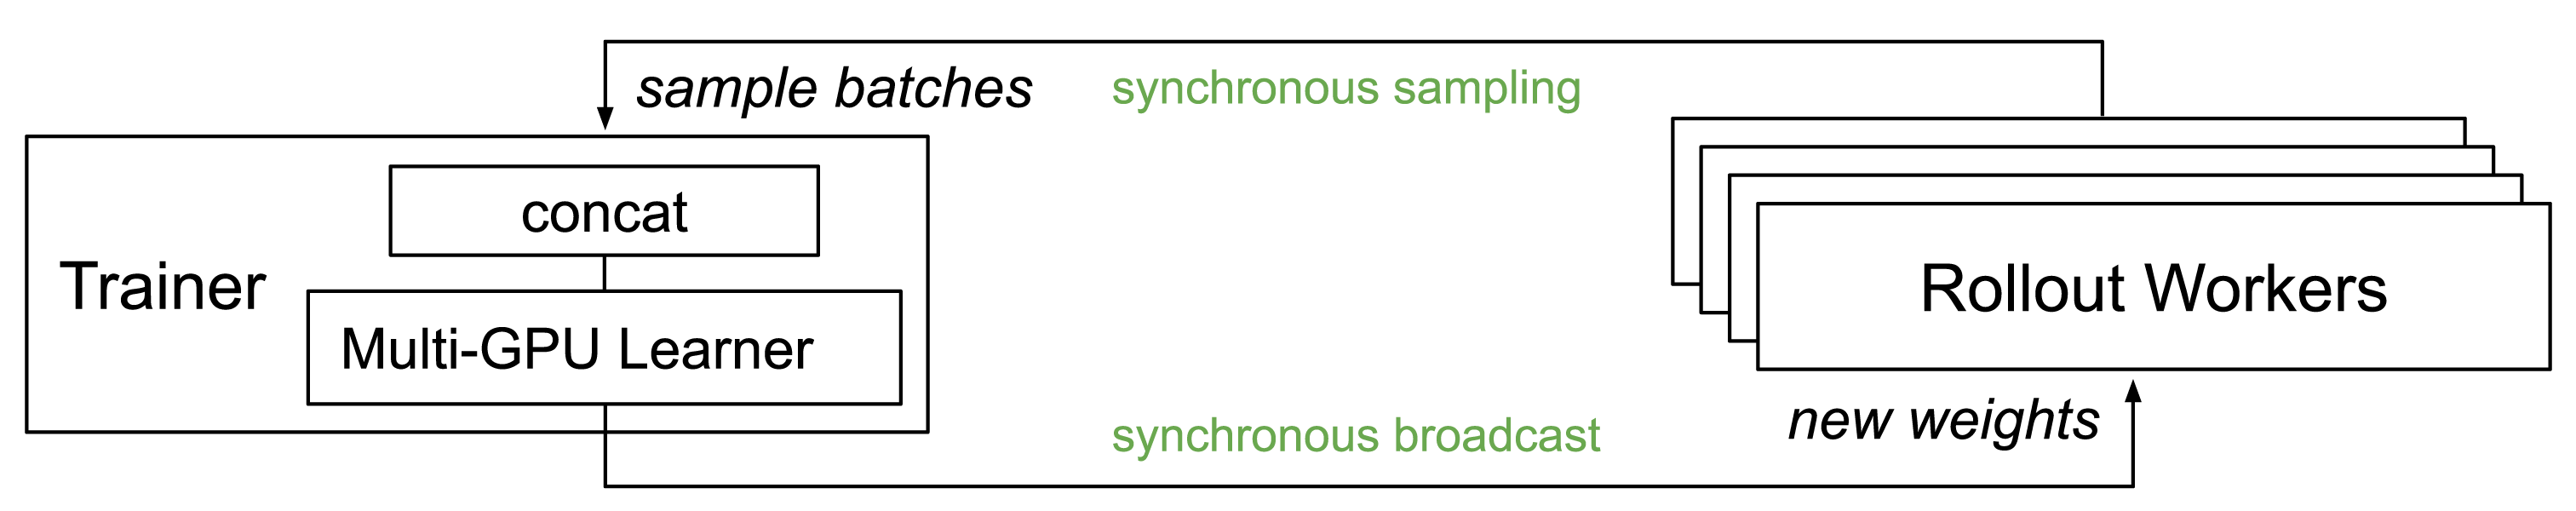
\includegraphics[scale=0.6]{gambar/rllib_ppo_architecture.png}
    % Keterangan gambar yang diinputkan
    \caption{Arsitektur PPO pada RLlib 2.0.0 \citep{rllibDocumentation}}
    % Label referensi dari gambar yang diinputkan
    \label{fig:rllib_ppo_architecture}
\end{figure}

\begin{lstlisting}[
  language=Python,
  caption={PPO-specific configs},
  label={lst:ppoSpecificConfigs}
]
# PPO specific settings:
self.lr_schedule = None
self.use_critic = True
self.use_gae = True
self.lambda_ = 1.0
self.kl_coeff = 0.2
self.sgd_minibatch_size = 128
self.num_sgd_iter = 30
self.shuffle_sequences = True
self.vf_loss_coeff = 1.0
self.entropy_coeff = 0.0
self.entropy_coeff_schedule = None
self.clip_param = 0.3
self.vf_clip_param = 10.0
self.grad_clip = None
self.kl_target = 0.01

# Override some of AlgorithmConfig's default values with PPO-specific values.
self.rollout_fragment_length = 200
self.train_batch_size = 4000
self.lr = 5e-5
self.model["vf_share_layers"] = False
    
\end{lstlisting}

\subsection{Implementasi IMPALA}
Implementasi IMPALA dari RLlib 2.0.0 menggunakan referensi kode V-trace milik DeepMind \citep{impala}.
Seperti APE-X DQN, IMPALA merupakan sebuah arsitektur terdistribusi. Arsitektur IMPALA juga mirip dengan PPO.
Akan tetapi, PPO menggunakan \emph{synchronous broadcast}, sedangkan IMPALA menggunakan \emph{asynchronous broadcast}.

\begin{figure}[H]
  \centering
    % Nama dari file gambar yang diinputkan
    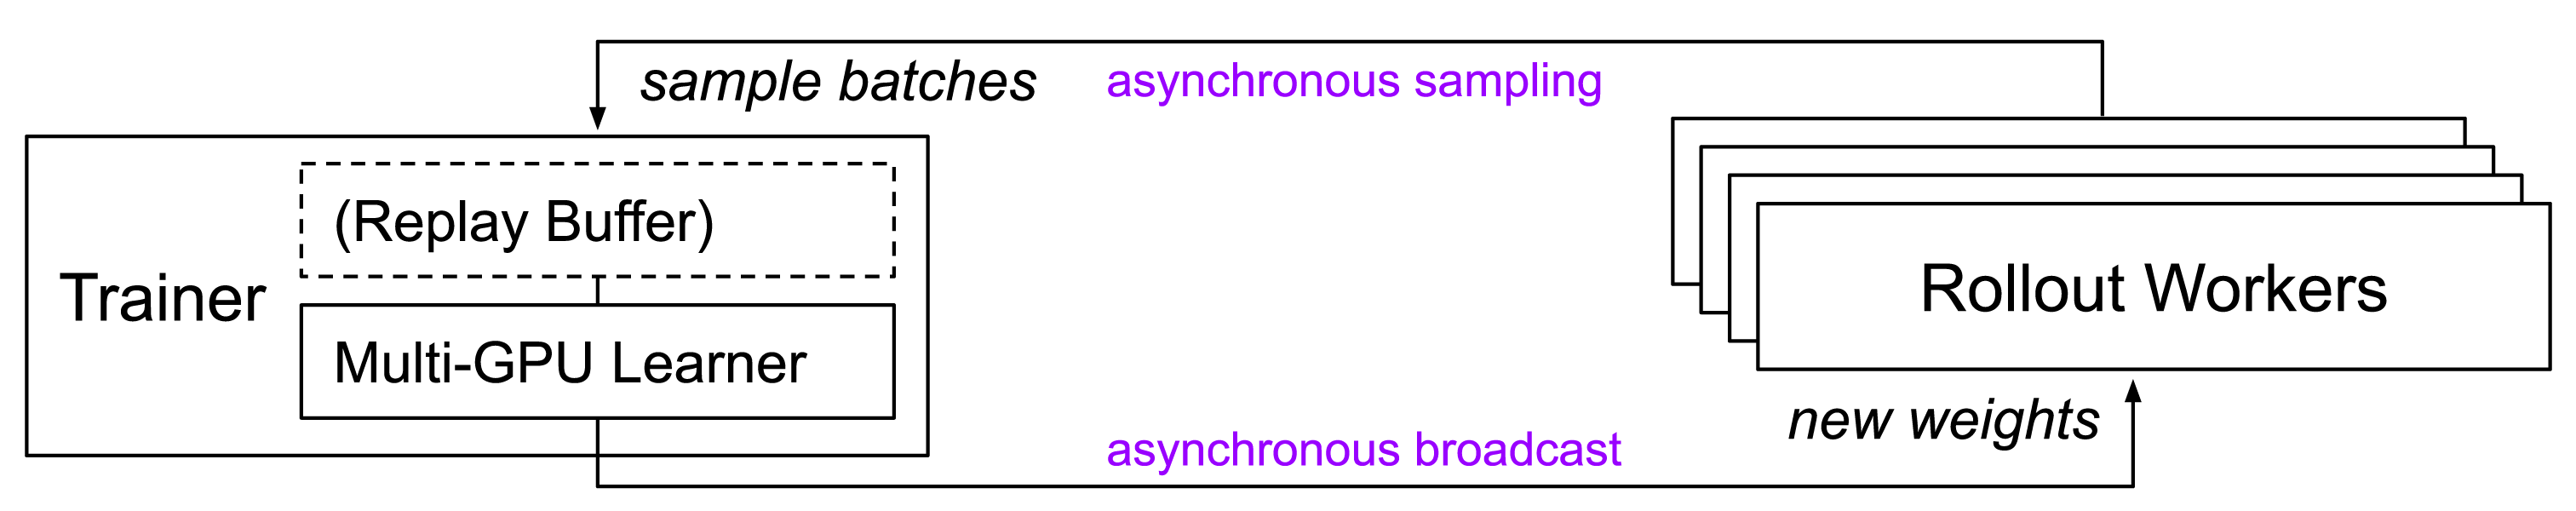
\includegraphics[scale=0.6]{gambar/rllib_impala_architecture.png}
    % Keterangan gambar yang diinputkan
    \caption{Arsitektur IMPALA pada RLlib 2.0.0 \citep{rllibDocumentation}}
    % Label referensi dari gambar yang diinputkan
    \label{fig:rllib_impala_architecture}
\end{figure}

\begin{lstlisting}[
  language=Python,
  caption={IMPALA-specific configs},
  label={lst:impalaSpecificConfigs}
]
# IMPALA specific settings:
self.vtrace = True
self.vtrace_clip_rho_threshold = 1.0
self.vtrace_clip_pg_rho_threshold = 1.0
self.vtrace_drop_last_ts = True
self.num_multi_gpu_tower_stacks = 1
self.minibatch_buffer_size = 1
self.num_sgd_iter = 1
self.replay_proportion = 0.0
self.replay_ratio = ((1 / self.replay_proportion)
                     if self.replay_proportion > 0 else 0.0)
self.replay_buffer_num_slots = 0
self.learner_queue_size = 16
self.learner_queue_timeout = 300
self.max_requests_in_flight_per_sampler_worker = 2
self.max_requests_in_flight_per_aggregator_worker = 2
self.timeout_s_sampler_manager = 0.0
self.timeout_s_aggregator_manager = 0.0
self.broadcast_interval = 1
self.num_aggregation_workers = 0
self.grad_clip = 40.0
self.opt_type = "adam"
self.lr_schedule = None
self.decay = 0.99
self.momentum = 0.0
self.epsilon = 0.1
self.vf_loss_coeff = 0.5
self.entropy_coeff = 0.01
self.entropy_coeff_schedule = None
self._separate_vf_optimizer = False
self._lr_vf = 0.0005
self.after_train_step = None

# Override some of AlgorithmConfig's default values with ARS-specific values.
self.rollout_fragment_length = 50
self.train_batch_size = 500
self.num_workers = 2
self.num_gpus = 1
self.lr = 0.0005
self.min_time_s_per_iteration = 10
    
\end{lstlisting}
  \cleardoublepage

  % Bab 4 pengujian dan analisis
  \chapter{HASIL DAN PEMBAHASAN}
\label{chap:hasilpembahasan}

Pada bab ini dipaparkan hasil dari eksperimen yang dilakukan pada penelitian ini.
Hasil dari training berupa \emph{mean episode rewards} dari agen \emph{attacker} dan agen \emph{defender},
waktu training, rerata waktu inferensi, rerata waktu proses \emph{actions}, rerata waktu \emph{environment} menunggu,
rerata waktu pemrosesan observasi mentah, dan presentase penggunaan CPU serta RAM.

Hasil dari evaluasi berupa performa algoritma jika dilawankan dengan generasi sebelum dan sesudahnya,
serta evaluasi performa algoritma dalam skenario \emph{environment} yang berbeda berupa area lebih besar
(16x16).

\section{Hasil Training}

Dalam eksperimen RL, hal yang paling penting untuk diperhatikan adalah nilai \emph{rewards} (\emph{episode rewards}) yang didapatkan oleh agen
selama training. Performa agen RL dapat diukur dengan seberapa banyak reward yang telah didapatkan oleh agen.
Dari eksperimen yang telah dilakukan, didapatkan beberapa nilai \emph{rewards}, 
seperti \emph{mean episode rewards}, \emph{max episode rewards}, dan \emph{min episode rewards} untuk kedua agen dengan keempat algoritma yang diuji coba.
\emph{Mean episode rewards} merupakan rerata nilai \emph{rewards} yang didapatkan oleh agen selama satu episode.

Nilai \emph{mean episode rewards} menunjukan akan performa kedua agen saat training.
Agen \emph{attacker} yang berhasil mencapai nilai \emph{atttacker mean episode reward} sebesar 20 poin atau ke atas
merupakan agen attacker yang dapat secara konsisten menyelesaikan tujuannya, yaitu menghancurkan kota.
Hal ini karena \emph{reward} yang didapatkan oleh agen \emph{attacker} dalam menghancurkan kota adalah 20 poin.

Nilai \emph{max episode rewards} merupakan nilai tertinggi yang didapatkan oleh agen selama training berlangsung.
Sebaliknya, nilai \emph{min episode rewards} merupakan nilai terendah yang didapatkan oleh agen selama training.


\begin{table}[h]
  \centering
  \label{table:meanEpisodeReward}
  \caption{Tabel nilai akhir \emph{mean episode rewards} kedua agen}
  \begin{tabular}{|c|c|c|}
  \hline
  \textbf{Algorithm} & \textbf{\begin{tabular}[c]{@{}c@{}}Attacker Mean\\ Episode Reward\end{tabular}} & \textbf{\begin{tabular}[c]{@{}c@{}}Defender Mean\\ Episode Reward\end{tabular}} \\ \hline
  APE-X DQN           & 20.62                                                                           & 2.36                                                                            \\ \hline
  DQN                & 2.05                                                                            & 0.71                                                                            \\ \hline
  PPO                & -3.2                                                                            & -1.9                                                                            \\ \hline
  IMPALA             & 1.041                                                                           & 2.24                                                                            \\ \hline
  \end{tabular}
\end{table}

\subsection{Attacker Mean Episode Rewards}

\begin{figure}[H]
  \centering
    % Nama dari file gambar yang diinputkan
    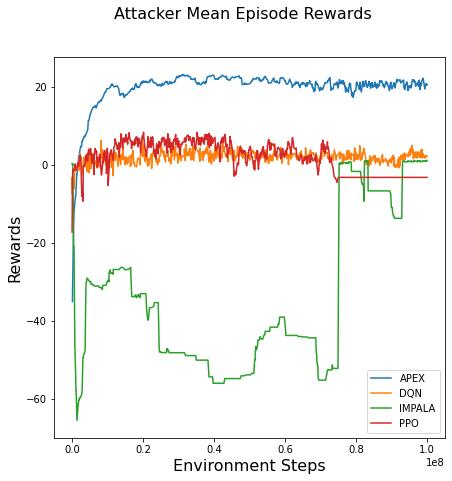
\includegraphics[scale=0.9]{gambar/attacker_reward_mean.jpg}
    % Keterangan gambar yang diinputkan
    \caption{Grafik menunjukan \emph{mean episode rewards} dari agen \emph{attacker}.
    Biru: APE-X DQN, oranye: DQN, hijau: IMPALA, merah: PPO}
    % Label referensi dari gambar yang diinputkan
    \label{fig:attackerMeanEpisodeGraph}
\end{figure}

Dari grafik \ref{fig:attackerMeanEpisodeGraph}, APE-X DQN merupakan algoritma yang paling baik,
jauh di atas algoritma lain. APE-X DQN mencapai nilai 20 poin sekitar pada 1.5 \emph{environment steps}.
APE-X DQN berkonvergensi di sekitar nilai 20 poin ini sebelum 2 juta \emph{environment steps}.
Mengingat 20 poin merupakan nilai \emph{reward} ketika agen \emph{attacker} menghancurkan kota,
agen \emph{attacker} APE-X DQN secara konsisten telah menyelesaikan tujuan tersebut.

Algoritma lain jauh dibawah performa APE-X DQN. Algoritma DQN selalu di bawah 5 poin dan tidak meningkat secara signifikan.
Algoritma PPO mencapai nilai 5 poin pada sekitar 1.5 juta \emph{environment steps}, akan tetapi menurun setelah 5 juta
\emph{environment steps}. PPO juga mengalami \emph{flatline} dimana secara tiba tiba algoritma tersebut
tidak mengalami peningkatan atau penurunan nilai \emph{rewards} pada sebelum 8 juta \emph{environment steps}
sampai akhir sesi. PPO merupakan algoritma terburuk pada grafik ini. IMPALA merupakan algoritma yang paling tidak stabil pada grafik ini.
Nilai \emph{mean episode rewards} agen \emph{attacker} IMPALA selalu di bawah -20 poin sampai
sekitar sebelum 8 juta \emph{environment steps} dimana IMPALA melonjak ke nilai 0 poin.
Nilai poin negatif dari IMPALA hanya bisa dicapai jika \emph{unit} agen \emph{attacker} mencoba untuk keluar
dari batas \emph{environment} secara terus menerus.

\subsection{Defender Mean Episode Rewards}

\begin{figure}[H]
  \centering
    % Nama dari file gambar yang diinputkan
    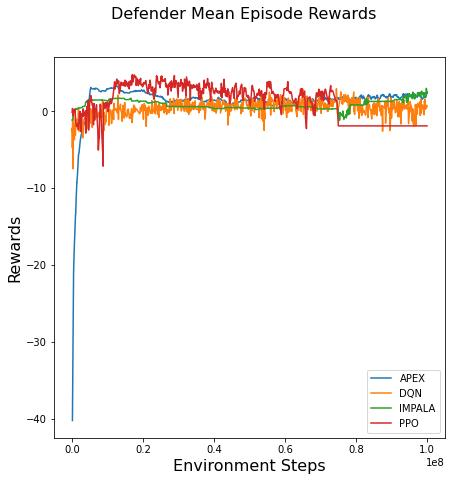
\includegraphics[scale=0.9]{gambar/defender_reward_mean.jpg}
    % Keterangan gambar yang diinputkan
    \caption{Grafik menunjukan \emph{mean episode rewards} dari agen \emph{defender}.
    Biru: APE-X DQN, oranye: DQN, hijau: IMPALA, merah: PPO}
    % Label referensi dari gambar yang diinputkan
    \label{fig:defenderMeanEpisodeGraph}
\end{figure}

Perubahan nilai \emph{rewards} algoritma dalam grafik \ref{fig:defenderMeanEpisodeGraph} jauh lebih stabil.
Hal ini disebabkan karena nilai \emph{general reward} yang diterima oleh agen \emph{defender} tidak memiliki varian yang tinggi,
dibandingkan dengan agen \emph{attacker} yang memerima 20 poin ketika menghancurkan kota.

APE-X DQN memulai dengan -40 poin akan tetapi secara cepat melonjak ke atas 2 poin.
Sama dengan di grafik \ref{fig:attackerMeanEpisodeGraph}, APE-X DQN merupakan algoritma paling stabil.
APE-X DQN juga salah satu algoritma dengan performa terbaik, bersebelahan dengan IMPALA.

DQN tidak berhasil melakukan konvergensi dengan baik dan nilainya tidak stabil sampai akhir sesi.
PPO juga merupakan algoritma terburuk pada grafik ini. Keadaan \emph{flatline} sama yang dialami PPO pada grafik
\ref{fig:attackerMeanEpisodeGraph} juga dapat dilihat disini.

\subsection{Attacker Min dan Max Episode Rewards}
\begin{table}[H]
  \centering
  \caption{Tabel nilai min dan max \emph{episode rewards} agen \emph{attacker}}
  \label{table:attackerMinMaxRewards}
  \begin{tabular}{|c|c|c|}
  \hline
  \textbf{Algorithm} & \textbf{\begin{tabular}[c]{@{}c@{}}Attacker Min\\ Episode Reward\end{tabular}} & \textbf{\begin{tabular}[c]{@{}c@{}}Attacker Max\\ Episode Reward\end{tabular}} \\ \hline
  APE-X DQN           & -0.9                                                                           & 30                                                                             \\ \hline
  DQN                & -15.4                                                                          & 25.2                                                                           \\ \hline
  PPO                & 0                                                                              & 2.8                                                                            \\ \hline
  IMPALA             & -26.2                                                                          & 14                                                                             \\ \hline
  \end{tabular}
\end{table}

Dari nilai \emph{max episode rewards} APE-X DQN merupakan algoritma tertinggi paka 30 poin.
Diikuti oleh DQN pada 25.2 poin.
Kedua algoritma ini berada di atas 20 poin, yang berarti bahwa agen \emph{attacker} pada algoritma tersebut
berhasil menghancurkan kota dalam salah satu episodenya.
30 poin pada APE-X DQN menunjukan bahwa APE-X DQN dapat menghancurkan kota dan sekaligus membunuh seluruh unit agen
defender pada salah satu episodenya.
30 poin merupakan poin yang hampir paling tinggi untuk bisa dicapai.
IMPALA mendapatkan 14 poin, yang berarti agen \emph{attacker} algoritma ini dapat menghancurkan kota dalam salah satu episodenya,
namun melakukannya dengan giliran yang lebih banyak dibandingkan DQN atau APE-X DQN.
PPO memiliki nilai max hanya sebesar 2.8 menunjukan bahwa agen \emph{attacker} PPO berhasil menghancurkan kota namun memerlukan hampir seluruh giliran yang ada.

Nilai \emph{min episode rewards} menunjukan performa terburuk agen \emph{attacker} pada salah satu episode.
PPO merupakan algoritma yang memiliki nilai minimum tertinggi sebesar 0.
Jika dibandingkan dengan nilai maksimum milik PPO, PPO merupakan algoritma yang cukup stabil karena perbedaan antara
minimum dan maksimum sangat kecil.
APE-X DQN merupakan algoritma kedua terbaik denga minimum sebesar -0.9, diikuti oleh DQN pada -15.4 dan IMPALA -26.2.

\subsection{Defender Min dan Max Episode Rewards}

\begin{table}[H]
  \centering
  \caption{Tabel nilai min dan max \emph{episode rewards} agen \emph{defender}}
  \label{table:defenderMinMaxRewards}
  \begin{tabular}{|c|c|c|}
  \hline
  \textbf{Algorithm} & \textbf{\begin{tabular}[c]{@{}c@{}}Defender Min\\ Episode Reward\end{tabular}} & \textbf{\begin{tabular}[c]{@{}c@{}}Defender Max\\ Episode Reward\end{tabular}} \\ \hline
  APE-X DQN           & 0                                                                              & 9.2                                                                            \\ \hline
  DQN                & -11.8                                                                          & 10.7                                                                           \\ \hline
  PPO                & -24.2                                                                          & 7.5                                                                            \\ \hline
  IMPALA             & -2.2                                                                           & 8.6                                                                            \\ \hline
  \end{tabular}
\end{table}

Pada nilai \emph{max episode rewards} agen \emph{defender}, seluruh algoritma memiliki nilai yang tidak jauh berbeda antara satu sama lain.
DQN menungguli algoritma lain pada nilai 10l7, diikuti oleh APE-X DQN pada 9.2, IMPALA 8.6 dan terakhir PPO pada 7.5.
Agen \emph{defender} seluruh algoritma dapat membunuh beberapa atau seluruh unit milik agen \emph{attacker} pada salah satu episodenya.
Maka performa terbaik dari seluruh algoritma hampir sama antar satu sama lain.

Pada nilai \emph{min episode rewards} agen \emph{defender}, APE-X DQN merupakan algoritma dengan nilai minimum tertinggi.
Nilai 0 yang didapatkan merupakan keadaan dimana agen \emph{defender} tidak melakukan banyak kesalahan pergerakan (bergerak ke ujung area)
atau dapat mengkompensasi kesalahan tersebut dengan membunuh beberapa unit lawan.
Berbalik dengan agen \emph{attacker}, IMPALA merupakan algoritma yang paling stabil dalam perbedaan nilai minimum dan maksimum.
Sedangkan PPO tidak sestabil nilai maksimum dan minimum agen \emph{attacker}.
PPO merupakan algoritma dengan nilai minimum terendah.

\subsection{Waktu dan Pemakaian Resource Algoritma}

\begin{table}[H]
  \centering
  \caption{Training, Inference, Processing Time, and Resource Usage}
  \label{table:timeAndResourceSpent}
  \begin{tabular}{|l|l|l|l|l|}
      \hline
      \textbf{Metrics}                                                            & \textbf{APE-X DQN} & \textbf{DQN}     & \textbf{PPO}     & \textbf{IMPALA}  \\ \hline
      \begin{tabular}[c]{@{}l@{}}Total Training \\ Time\end{tabular}          & 1d 17h             & 8d 7h            & 3d 3h             & 23h     \\ \hline
      \begin{tabular}[c]{@{}l@{}}Mean Inference \\ (ms)\end{tabular}          & 3.406     & 9.191   & 2.446   & 1.862   \\ \hline
      \begin{tabular}[c]{@{}l@{}}Mean Action \\ Processing (ms)\end{tabular}  & 0.06758   & 0.07171 & 0.05702 & 0.05636 \\ \hline
      \begin{tabular}[c]{@{}l@{}}Mean Environment \\ Wait (ms)\end{tabular}   & 0.457     & 0.4237  & 0.414   & 0.4119  \\ \hline
      \begin{tabular}[c]{@{}l@{}}Mean Raw Obs \\ Processing (ms)\end{tabular} & 0.3512    & 0.2834  & 0.2363  & 0.2143  \\ \hline
      RAM Utilization                                                         & 82.3\%    & 38.82\% & 36.1\%  & 33.2\%  \\ \hline
      CPU Utilization                                                         & 79.95\%   & 40.78\% & 39.63\% & 63.51\% \\ \hline
  \end{tabular}
\end{table}

Tabel \ref{table:timeAndResourceSpent} menunjukan bahwa IMPALA merupakan algoritma tercepat
untuk menyelesaikan 10 juta \emph{environment step} dengan \emph{total training time} selama
23 jam. APE-X DQN mengikuti IMPALA tidak jauh setelahnya dengan \emph{total training time}
selama 1 hari 7 jam (30 jam). PPO memerlukan waktu lebih dari 3x lebih lama dengan \emph{total training time}
sebesar 3 hari 3 jam (75 jam). DQN merupakan algoritma terlama yang memerlukan 8 hari 7 jam (199 jam).

IMPALA juga merupakan algoritma tercepat dalam inferensi dengan nilai \emph{mean inference} sebesar
1.862 ms. PPO merupakan algoritma tercepat kedua dengan \emph{mean inference} sebesar 2.446 ms walaupun \emph{total
training time} PPO lebih lambat dari APE-X DQN, APE-X DQN berada di setelah PPO dengan \emph{mean inference}
sebesar 3.406 ms. DQN merupakan algoritma terlama dalam melakukan inferensi dengan 9.191 ms.
\emph{Metrics} lainnya seperti \emph{mean action processing}, \emph{mean environment wait}, dan \emph{mean raw obs processing}
tidak berbeda jauh antara satu algoritma dengan algoritma lainnya.

Pada penggunaan RAM dan CPU, APE-X DQN merupakan algoritma yang menggunakan CPU dan RAM terbanyak
dengan penggunaan CPU sebesar 79.95\% dan RAM sebesar 82.3\%. Hal ini disebabkan oleh penggunaan CPU
APE-X DQN yang menggunakan seluruh 8 \emph{cores} dibandingkan algoritma lain yang menggunakan 4 \emph{cores}
dengan jumlah \emph{workers} yang sama (3 \emph{workers}). IMPALA merupakan algoritma DRL
terdistribusi lainnya yang menggunakan CPU terbanyak setelah APE-X DQN dengan penggunaan sebesar
63.51\%. Akan tetapi penggunaan RAM dari IMPALA jauh lebih minim dengan penggunaan sebesar 33.2\%.
PPO dan DQN menggunakan CPU dan RAM sama banyaknya dengan penggunaan CPU sebesar 39-40\% dan RAM
sebesar 36-39\%.

\section{Hasil Evaluasi}
Setelah dilakukan \emph{training}, terdapat dua macam evaluasi yang dilakukan.
Evaluasi antar generasi algoritma dan evaluasi dengan \emph{environment} yang lebih luas.
Hasil dari kedua evaluasi merupakan \emph{rewards} yang didapatkan oleh agen pada setiap generasi algoritma.
Evaluasi dimulai dari generasi 1 agen \emph{attakcer} melawan seluruh generasi dari agen \emph{defender}.
Kemudian dilanjut pada generasi 2 agen \emph{attacker} melawan seluruh generasi dari agen \emph{defender}.
Hingga seluruh generasi dari sebuah algoritma sudah melawan satu sama lain.

\subsection{Hasil Evaluasi Antar Generasi Algoritma}

\begin{table}[H]
  \centering
  \caption{Evaluasi Antar Generasi DQN}
  \label{table:dqnVersusResult}
  \begin{tabular}{|c|c|c|c|}
  \hline
  \textbf{\begin{tabular}[c]{@{}c@{}}Attacker Agent\\ Generation\end{tabular}} & \textbf{\begin{tabular}[c]{@{}c@{}}Defender Agent\\ Generation\end{tabular}} & \textbf{\begin{tabular}[c]{@{}c@{}}Attacker Mean\\ Episode Rewards\end{tabular}} & \textbf{\begin{tabular}[c]{@{}c@{}}Defender Mean\\ Episode Rewards\end{tabular}} \\ \hline
  \multirow{4}{*}{1}                                                           & 1                                                                            & -80.15                                                                           & -6.53                                                                            \\ \cline{2-4} 
                                                                               & 2                                                                            & -71.4                                                                            & -15.75                                                                           \\ \cline{2-4} 
                                                                               & 3                                                                            & -79.617                                                                          & -53.08                                                                           \\ \cline{2-4} 
                                                                               & 4                                                                            & -82.76                                                                           & -37.38                                                                           \\ \hline
  \multirow{4}{*}{2}                                                           & 1                                                                            & -0.46                                                                            & -18.46                                                                           \\ \cline{2-4} 
                                                                               & 2                                                                            & -0.56                                                                            & -13.53                                                                           \\ \cline{2-4} 
                                                                               & 3                                                                            & -0.41                                                                            & -48.12                                                                           \\ \cline{2-4} 
                                                                               & 4                                                                            & -0.66                                                                            & -27.16                                                                           \\ \hline
  \multirow{4}{*}{3}                                                           & 1                                                                            & -0.72                                                                            & -16.53                                                                           \\ \cline{2-4} 
                                                                               & 2                                                                            & -1.98                                                                            & -13.38                                                                           \\ \cline{2-4} 
                                                                               & 3                                                                            & -1.68                                                                            & -46.59                                                                           \\ \cline{2-4} 
                                                                               & 4                                                                            & -2.6                                                                             & -25.1                                                                            \\ \hline
  \multirow{4}{*}{4}                                                           & 1                                                                            & -0.71                                                                            & -15.78                                                                           \\ \cline{2-4} 
                                                                               & 2                                                                            & -0.65                                                                            & -11.86                                                                           \\ \cline{2-4} 
                                                                               & 3                                                                            & -1.30                                                                            & -48.36                                                                           \\ \cline{2-4} 
                                                                               & 4                                                                            & -0.52                                                                            & -28.56                                                                           \\ \hline
  \end{tabular}
\end{table}

Pada algoritma DQN, performa antar generasi agen \emph{attacker} memmiliki nilai \emph{mean episode rewards} yang mirip, kecuali generasi pertama.
Performa agen \emph{attacker} generasi 1 jauh dibawah performa generasi-generasi selanjutnya.
Ini merupakan salah satu dampak penggunaan \emph{epsilon greedy} dalam algoritma DQN.
Algoritma DQN akan melakukan aksi secara acak pada saat \emph{training} untuk melakukan eksplorasi.
Generasi pertama akan sering melakukan eksplorasi untuk mencari nilai \emph{Q-value} yang optimal
Generasi-generasi setelahnya melakukan \emph{exploitation} akan eksplorasi yang sudah dilakukan oleh generasi sebelumnya.
Untuk agen \emph{defender}, generasi 3 merupakan generasi yang paling buruk.
Generasi ke 3 memiliki nilai paling rendah saat melawan generasi manapun.

\begin{table}[H]
  \centering
  \caption{Evaluasi Antar Generasi APE-X DQN}
  \label{table:apexDqnVersusResult}
  \begin{tabular}{|c|c|c|c|}
  \hline
  \textbf{\begin{tabular}[c]{@{}c@{}}Attacker Agent\\ Generation\end{tabular}} & \textbf{\begin{tabular}[c]{@{}c@{}}Defender Agent\\ Generation\end{tabular}} & \textbf{\begin{tabular}[c]{@{}c@{}}Attacker Mean\\ Episode Rewards\end{tabular}} & \textbf{\begin{tabular}[c]{@{}c@{}}Defender Mean\\ Episode Rewards\end{tabular}} \\ \hline
  \multirow{4}{*}{1}                                                           & 1                                                                            & -14.33                                                                                                & -56.00                                                                                                \\ \cline{2-4} 
                                                                              & 2                                                                            & -25.50                                                                                                & -29.14                                                                                                \\ \cline{2-4} 
                                                                              & 3                                                                            & -11.74                                                                                                & -24.78                                                                                                \\ \cline{2-4} 
                                                                              & 4                                                                            & -16.30                                                                                                & 3.25                                                                                                  \\ \hline
  \multirow{4}{*}{2}                                                           & 1                                                                            & -6.88                                                                                                 & -49.60                                                                                                \\ \cline{2-4} 
                                                                              & 2                                                                            & -65.80                                                                                                & -53.00                                                                                                \\ \cline{2-4} 
                                                                              & 3                                                                            & -2.66                                                                                                 & 1.65                                                                                                  \\ \cline{2-4} 
                                                                              & 4                                                                            & -2.19                                                                                                 & -3.21                                                                                                 \\ \hline
  \multirow{4}{*}{3}                                                           & 1                                                                            & 4.54                                                                                                  & -52.10                                                                                                \\ \cline{2-4} 
                                                                              & 2                                                                            & 7.02                                                                                                  & -7.23                                                                                                 \\ \cline{2-4} 
                                                                              & 3                                                                            & 6.34                                                                                                  & 2.11                                                                                                  \\ \cline{2-4} 
                                                                              & 4                                                                            & 5.50                                                                                                  & 3.26                                                                                                  \\ \hline
  \multirow{4}{*}{4}                                                           & 1                                                                            & 13.80                                                                                                 & -20.82                                                                                                \\ \cline{2-4} 
                                                                              & 2                                                                            & 10.50                                                                                                 & -2.00                                                                                                 \\ \cline{2-4} 
                                                                              & 3                                                                            & 12.20                                                                                                 & 2.55                                                                                                  \\ \cline{2-4} 
                                                                              & 4                                                                            & 11.70                                                                                                 & 3.11                                                                                                  \\ \hline
  \end{tabular}
\end{table}

Algoritma APE-X DQN memiliki awal yang mirip dengan DQN, dimana nilai \emph{mean episode rewards} sangat kecil pada generasi awal.
Hal ini karena APE-X DQN juga menggunakan \emph{epsilon greedy} untuk eksplorasi dan eksploitasi nilai \emph{Q-value}.
Namun, dapat dilihat bahwa nilai \emph{episode mean rewards} kedua agen meningkat pada setiap generasi.
Agen \emph{attacker} mampu mendapatkan nilai di atas sepuluh pada generasi ke empat.

\begin{table}[H]
  \centering
  \caption{Evaluasi Antar Generasi PPO}
  \label{table:ppoVersusResult}
  \begin{tabular}{|c|c|c|c|}
  \hline
  \textbf{\begin{tabular}[c]{@{}c@{}}Attacker Agent\\ Generation\end{tabular}} & \textbf{\begin{tabular}[c]{@{}c@{}}Defender Agent\\ Generation\end{tabular}} & \textbf{\begin{tabular}[c]{@{}c@{}}Attacker Mean\\ Episode Rewards\end{tabular}} & \textbf{\begin{tabular}[c]{@{}c@{}}Defender Mean\\ Episode Rewards\end{tabular}} \\ \hline
  \multirow{4}{*}{1}                                                           & 1                                                                            & -80.15                                                                           & -6.53                                                                            \\ \cline{2-4} 
                                                                               & 2                                                                            & -71.4                                                                            & -15.75                                                                           \\ \cline{2-4} 
                                                                               & 3                                                                            & -79.617                                                                          & -53.08                                                                           \\ \cline{2-4} 
                                                                               & 4                                                                            & -82.76                                                                           & -37.38                                                                           \\ \hline
  \multirow{4}{*}{2}                                                           & 1                                                                            & -0.46                                                                            & -18.46                                                                           \\ \cline{2-4} 
                                                                               & 2                                                                            & -0.56                                                                            & -13.53                                                                           \\ \cline{2-4} 
                                                                               & 3                                                                            & -0.41                                                                            & -48.12                                                                           \\ \cline{2-4} 
                                                                               & 4                                                                            & -0.66                                                                            & -27.16                                                                           \\ \hline
  \multirow{4}{*}{3}                                                           & 1                                                                            & -0.72                                                                            & -16.53                                                                           \\ \cline{2-4} 
                                                                               & 2                                                                            & -1.98                                                                            & -13.38                                                                           \\ \cline{2-4} 
                                                                               & 3                                                                            & -1.68                                                                            & -46.59                                                                           \\ \cline{2-4} 
                                                                               & 4                                                                            & -2.6                                                                             & -25.1                                                                            \\ \hline
  \multirow{4}{*}{4}                                                           & 1                                                                            & -0.71                                                                            & -15.78                                                                           \\ \cline{2-4} 
                                                                               & 2                                                                            & -0.65                                                                            & -11.86                                                                           \\ \cline{2-4} 
                                                                               & 3                                                                            & -1.30                                                                            & -48.36                                                                           \\ \cline{2-4} 
                                                                               & 4                                                                            & -0.52                                                                            & -28.56                                                                           \\ \hline
  \end{tabular}
\end{table}

Sama seperti APE-X DQN, agen \emph{attacker} PPO mendapatkan peningkatan pada setiap generasi.
Akan tetapi, peningkatan yang dialami oleh PPO tidak sesignifikan peningkatan pada algoritma APE-X DQN.
Dimana generasi 4 adalah generasi terbaik untuk agen \emph{attacker}, generasi 2 merupakan generasi terbaik untuk agen \emph{defender}.

\begin{table}[H]
  \centering
  \caption{Evaluasi Antar Generasi IMPALA}
  \label{table:impalaVersusResult}
  \begin{tabular}{|c|c|l|l|}
  \hline
  \textbf{\begin{tabular}[c]{@{}c@{}}Attacker Agent\\ Generation\end{tabular}} & \textbf{\begin{tabular}[c]{@{}c@{}}Defender Agent\\ Generation\end{tabular}} & \textbf{\begin{tabular}[c]{@{}c@{}}Attacker Mean\\ Episode Rewards\end{tabular}} & \textbf{\begin{tabular}[c]{@{}c@{}}Defender Mean\\ Episode Rewards\end{tabular}} \\ \hline
  \multirow{4}{*}{1}                                                           & 1                                                                            & -0.84                                                                            & -15.23                                                                           \\ \cline{2-4} 
                                                                               & 2                                                                            & -0.99                                                                            & -44.74                                                                           \\ \cline{2-4} 
                                                                               & 3                                                                            & -0.67                                                                            & -47.81                                                                           \\ \cline{2-4} 
                                                                               & 4                                                                            & -1.16                                                                            & -49.33                                                                           \\ \hline
  \multirow{4}{*}{2}                                                           & 1                                                                            & 0.01                                                                             & -15.07                                                                           \\ \cline{2-4} 
                                                                               & 2                                                                            & 0.19                                                                             & -46.16                                                                           \\ \cline{2-4} 
                                                                               & 3                                                                            & 0.24                                                                             & -50.66                                                                           \\ \cline{2-4} 
                                                                               & 4                                                                            & 0.14                                                                             & -52.48                                                                           \\ \hline
  \multirow{4}{*}{3}                                                           & 1                                                                            & 0.02                                                                             & -14.88                                                                           \\ \cline{2-4} 
                                                                               & 2                                                                            & 0.26                                                                             & -44.34                                                                           \\ \cline{2-4} 
                                                                               & 3                                                                            & 0.27                                                                             & -50.12                                                                           \\ \cline{2-4} 
                                                                               & 4                                                                            & 0.25                                                                             & -50.88                                                                           \\ \hline
  \multirow{4}{*}{4}                                                           & 1                                                                            & 0.01                                                                             & -15.63                                                                           \\ \cline{2-4} 
                                                                               & 2                                                                            & 0.32                                                                             & -43.77                                                                           \\ \cline{2-4} 
                                                                               & 3                                                                            & 0.27                                                                             & -49.95                                                                           \\ \cline{2-4} 
                                                                               & 4                                                                            & 0.19                                                                             & -50.94                                                                           \\ \hline
  \end{tabular}
\end{table}

Berbeda dengan saat training, IMPALA merupakan algoritma yang paling stabil dalam evaluasi.
Namun peningkatan performa antar generasi algoritma IMPALA sangatlah kecil.
Agen \emph{defender} IMPALA juga tidak memiliki nilai \emph{mean episode rewards} yang baik pada seluruh generasi
dengan generasi terbaik berupa generasi 1 yang mempunyai nilai sekitar -15 poin.

\subsection{Hasil Evaluasi dengan Environment Lebih Luas}

Hasil pada algoritma APE-X DQN dan PPO tidak memiliki hasil lengkap. 
Hal ini dikarenakan dua model tersebut yang macet menjalankan evaluasi setelah beberapa generasi.
Sampai saat ini, solusi untuk masalah ini belum ditemukan dan akan dikomunikasikan ke pengembang RLlib.
Karena proses training ulang yang memakan waktu lama, maka generasi tersebut tidak dievaluasi.
Generasi yang tidak dapat dievaluasi diberi nilai n/a.

\begin{table}[H]
  \centering
  \caption{Evaluasi \emph{Environment} 16x16 DQN}
  \label{table:dqn16x16Result}
  \begin{tabular}{|c|c|c|c|}
  \hline
  \textbf{\begin{tabular}[c]{@{}c@{}}Attacker Agent\\ Generation\end{tabular}} & \textbf{\begin{tabular}[c]{@{}c@{}}Defender Agent\\ Generation\end{tabular}} & \textbf{\begin{tabular}[c]{@{}c@{}}Attacker Mean\\ Episode Rewards\end{tabular}} & \textbf{\begin{tabular}[c]{@{}c@{}}Defender Mean\\ Episode Rewards\end{tabular}} \\ \hline
    \multirow{4}{*}{1}                                                           & 1                                                                            & -69.43                                                                           & -1.77                                                                            \\ \cline{2-4} 
    & 2                                                                            & -64.34                                                                           & -11.53                                                                           \\ \cline{2-4} 
    & 3                                                                            & -70.40                                                                           & -47.10                                                                           \\ \cline{2-4} 
    & 4                                                                            & -75.41                                                                           & -29.30                                                                           \\ \hline
  \multirow{4}{*}{2}                                                           & 1                                                                            & -0.05                                                                            & -25.84                                                                           \\ \cline{2-4} 
    & 2                                                                            & -0.86                                                                            & -14.11                                                                           \\ \cline{2-4} 
    & 3                                                                            & -0.70                                                                            & -35.89                                                                           \\ \cline{2-4} 
    & 4                                                                            & -0.20                                                                            & -14.15                                                                           \\ \hline
  \multirow{4}{*}{3}                                                           & 1                                                                            & -2.92                                                                            & -26.21                                                                           \\ \cline{2-4} 
    & 2                                                                            & -4.98                                                                            & -9.48                                                                            \\ \cline{2-4} 
    & 3                                                                            & -2.74                                                                            & -39.40                                                                           \\ \cline{2-4} 
    & 4                                                                            & -2.56                                                                            & -14.52                                                                           \\ \hline
  \multirow{4}{*}{4}                                                           & 1                                                                            & -0.36                                                                            & -24.76                                                                           \\ \cline{2-4} 
    & 2                                                                            & -0.32                                                                            & -11.90                                                                           \\ \cline{2-4} 
    & 3                                                                            & -0.50                                                                            & -37.53                                                                           \\ \cline{2-4} 
    & 4                                                                            & -0.29                                                                            & -16.09                                                                           \\ \hline
  \end{tabular}
\end{table}

Nilai \emph{mean episode rewards} yang didapatkan saat evaluasi ini agak berbeda dengan evaluasi antar generasi.
Jenis generasi yang unggul dalam suatu agen berbeda dengan sebelumnya.
Agen \emph{attacker} memiliki generasi 2 sebagai generasi terbaik, sedikit lebih baik daripada generasi 4.
Untuk agen \emph{defender}, generasi ke 2 juga merupakan generasi yang memiliki nilai tertinggi.

\begin{table}[H]
  \centering
  \caption{Evaluasi \emph{Environment} 16x16 APE-X DQN}
  \label{table:apexDqn16x16Result}
  \begin{tabular}{|c|c|c|c|}
  \hline
  \textbf{\begin{tabular}[c]{@{}c@{}}Attacker Agent\\ Generation\end{tabular}} & \textbf{\begin{tabular}[c]{@{}c@{}}Defender Agent\\ Generation\end{tabular}} & \textbf{\begin{tabular}[c]{@{}c@{}}Attacker Mean\\ Episode Rewards\end{tabular}} & \textbf{\begin{tabular}[c]{@{}c@{}}Defender Mean\\ Episode Rewards\end{tabular}} \\ \hline
  \multirow{4}{*}{1}                                                           & 1                                                                            & -91.00                                                                           & -53.00                                                                           \\ \cline{2-4} 
    & 2                                                                            & -74.00                                                                           & -53.00                                                                           \\ \cline{2-4} 
    & 3                                                                            & -79.00                                                                           & -53.00                                                                           \\ \cline{2-4} 
    & 4                                                                            & n/a                                                                              & n/a                                                                              \\ \hline
  \multirow{4}{*}{2}                                                           & 1                                                                            & n/a                                                                              & n/a                                                                              \\ \cline{2-4} 
    & 2                                                                            & n/a                                                                              & n/a                                                                              \\ \cline{2-4} 
    & 3                                                                            & n/a                                                                              & n/a                                                                              \\ \cline{2-4} 
    & 4                                                                            & n/a                                                                              & n/a                                                                              \\ \hline
  \multirow{4}{*}{3}                                                           & 1                                                                            & n/a                                                                              & n/a                                                                              \\ \cline{2-4} 
    & 2                                                                            & n/a                                                                              & n/a                                                                              \\ \cline{2-4} 
    & 3                                                                            & n/a                                                                              & n/a                                                                              \\ \cline{2-4} 
    & 4                                                                            & n/a                                                                              & n/a                                                                              \\ \hline
  \multirow{4}{*}{4}                                                           & 1                                                                            & n/a                                                                              & n/a                                                                              \\ \cline{2-4} 
    & 2                                                                            & n/a                                                                              & n/a                                                                              \\ \cline{2-4} 
    & 3                                                                            & n/a                                                                              & n/a                                                                              \\ \cline{2-4} 
    & 4                                                                            & n/a                                                                              & n/a                                                                              \\ \hline
  \end{tabular}
\end{table}

Karena keterbatasan waktu evaluasi, tidak seluruh generasi APE-X DQN dapat dievaluasi.
Selama generasi 1, agen \emph{attacker} terlihat lebih stabil daripada saat evaluasi sebelumnya.
Berbeda dengan evaluasi sebelumnya, generasi 1 dari agen \emph{attacker} APE-X DQN memiliki nilai \emph{mean reward} yang lebih besar.
Generasi 1 APE-X DQN dalam evaluasi ini merupakan generasi terbaik untuk kedua agen.


\begin{table}[H]
  \centering
  \caption{Evaluasi \emph{Environment} 16x16 PPO}
  \label{table:ppo16x16Result}
  \begin{tabular}{|c|c|c|c|}
  \hline
  \textbf{\begin{tabular}[c]{@{}c@{}}Attacker Agent\\ Generation\end{tabular}} & \textbf{\begin{tabular}[c]{@{}c@{}}Defender Agent\\ Generation\end{tabular}} & \textbf{\begin{tabular}[c]{@{}c@{}}Attacker Mean\\ Episode Rewards\end{tabular}} & \textbf{\begin{tabular}[c]{@{}c@{}}Defender Mean\\ Episode Rewards\end{tabular}} \\ \hline
  \multirow{4}{*}{1}                                                           & 1                                                                            & 0.22                                                                             & -0.06                                                                            \\ \cline{2-4} 
    & 2                                                                            & 0.06                                                                             & -40.69                                                                           \\ \cline{2-4} 
    & 3                                                                            & -0.06                                                                            & -7.54                                                                            \\ \cline{2-4} 
    & 4                                                                            & -0.01                                                                            & -2.87                                                                            \\ \hline
  \multirow{4}{*}{2}                                                           & 1                                                                            & n/a                                                                              & n/a                                                                              \\ \cline{2-4} 
    & 2                                                                            & n/a                                                                              & n/a                                                                              \\ \cline{2-4} 
    & 3                                                                            & n/a                                                                              & n/a                                                                              \\ \cline{2-4} 
    & 4                                                                            & n/a                                                                              & n/a                                                                              \\ \hline
  \multirow{4}{*}{3}                                                           & 1                                                                            & n/a                                                                              & n/a                                                                              \\ \cline{2-4} 
    & 2                                                                            & n/a                                                                              & n/a                                                                              \\ \cline{2-4} 
    & 3                                                                            & n/a                                                                              & n/a                                                                              \\ \cline{2-4} 
    & 4                                                                            & n/a                                                                              & n/a                                                                              \\ \hline
  \multirow{4}{*}{4}                                                           & 1                                                                            & n/a                                                                              & n/a                                                                              \\ \cline{2-4} 
    & 2                                                                            & n/a                                                                              & n/a                                                                              \\ \cline{2-4} 
    & 3                                                                            & n/a                                                                              & n/a                                                                              \\ \cline{2-4} 
    & 4                                                                            & n/a                                                                              & n/a                                                                              \\ \hline
  \end{tabular}
\end{table}

Evaluasi pada setiap generasi juga tidak dapat dilakukan pada algoritma PPO karena masalah yang sama dengan APE-X DQN.
Evaluasi yang dapat dilakukan adalah generasi 1 agen \emph{attacker} melawan seluruh generasi agen \emph{defender}
Algoritma PPO memiliki perubahan yang stabil dalam evaluasi ini.
Pengecualian pada generasi 2 untuk agen \emph{defender} yang memiliki nilai -40.

\begin{table}[H]
  \centering
  \caption{Evaluasi \emph{Environment} 16x16 IMPALA}
  \label{table:impala16x16Result}
  \begin{tabular}{|c|c|l|l|}
  \hline
  \textbf{\begin{tabular}[c]{@{}c@{}}Attacker Agent\\ Generation\end{tabular}} & \textbf{\begin{tabular}[c]{@{}c@{}}Defender Agent\\ Generation\end{tabular}} & \multicolumn{1}{c|}{\textbf{\begin{tabular}[c]{@{}c@{}}Attacker Mean\\ Episode Rewards\end{tabular}}} & \multicolumn{1}{c|}{\textbf{\begin{tabular}[c]{@{}c@{}}Defender Mean\\ Episode Rewards\end{tabular}}} \\ \hline
  \multirow{4}{*}{1}                                                           & 1                                                                            & -0.49                                                                                                 & -10.37                                                                                                \\ \cline{2-4} 
    & 2                                                                            & -0.31                                                                                                 & -38.20                                                                                                \\ \cline{2-4} 
    & 3                                                                            & -0.46                                                                                                 & -43.53                                                                                                \\ \cline{2-4} 
    & 4                                                                            & -0.45                                                                                                 & -45.54                                                                                                \\ \hline
  \multirow{4}{*}{2}                                                           & 1                                                                            & 0.01                                                                                                  & -10.81                                                                                                \\ \cline{2-4} 
    & 2                                                                            & 0.23                                                                                                  & -40.28                                                                                                \\ \cline{2-4} 
    & 3                                                                            & 0.24                                                                                                  & -43.05                                                                                                \\ \cline{2-4} 
    & 4                                                                            & 0.23                                                                                                  & -44.56                                                                                                \\ \hline
  \multirow{4}{*}{3}                                                           & 1                                                                            & 0.02                                                                                                  & -10.39                                                                                                \\ \cline{2-4} 
    & 2                                                                            & 0.21                                                                                                  & -40.10                                                                                                \\ \cline{2-4} 
    & 3                                                                            & 0.19                                                                                                  & -45.20                                                                                                \\ \cline{2-4} 
    & 4                                                                            & 0.28                                                                                                  & -44.28                                                                                                \\ \hline
  \multirow{4}{*}{4}                                                           & 1                                                                            & 0.01                                                                                                  & -9.96                                                                                                 \\ \cline{2-4} 
    & 2                                                                            & 0.21                                                                                                  & -40.03                                                                                                \\ \cline{2-4} 
    & 3                                                                            & 0.15                                                                                                  & -45.14                                                                                                \\ \cline{2-4} 
    & 4                                                                            & 0.23                                                                                                  & -44.89                                                                                                \\ \hline
  \end{tabular}
\end{table}

Nilai \emph{episode mean rewards} dari algoritma IMPALA tidak jauh berbeda dari evaluasi sebelumnya.
Kestabilan dari nilai juga masih terlihat dalam evaluasi ini.
Generasi terbaik untuk agen \emph{attacker} IMPALA tidak cukup jelas.
Akan tetapi generasi 1 merupakan generasi paling buruk.
Untuk agen \emph{defender}, generasi 1 merupakan generasi terbaik.
Generasi lainnya memiliki nilai yang mirip antara satu dengan yang lain.

\section{Masalah Saat Evaluasi APE-X DQN dan PPO}
Pada saat evaluasi, algoritma APE-X DQN dan PPO tidak dapat sepenuhnya dijalankan pada seluruh generasi.
Generasi yang bermasalah adalah generasi 2 dan ke atas agen \emph{defender} untuk kedua algoritma.
Algoritma tersebut dapat berjalan, hanya saja waktu inferensi pada generasi tersebut yang tidak seperti biasanya.

Dalam evaluasi sebuah generasi, biasanya diperlukan waktu kurang dari sepuluh menit.
Maka satu algoritma setidaknya akan menyelesaikan evaluasi dalam waktu kurang dari satu jam.
Namun dalam menjalankan evaluasi agen \emph{attacker} APE-X DQN dan PPO generasi 2, evaluasi berjalan selama lebih dari 8 jam.
Sedangkan progress yang didapatkan dalam 8 jam tersebut nihil.

M dicoba seperti menurunkan jumlah iterasi menjadi satu episode per generasi tidak sepenuhnya menyelesaikan masalah ini.
Saat diubah menjadi satu episode per generasi, generasi yang bermasalah merupakan generasi 3 dan 4.
Karena keterbatasan waktu, maka tidak memungkinkan dilakukan training ulang untuk bobot dari generasi algoritma ini.
Adanya juga kemungkinan ini adalah sebuah \emph{bug} dalam RLlib.
Akan perlu dikomunikasikan lebih lanjut ke pengembang \emph{RLlib} untuk melakukan konfirmasi atas masalah ini.

  \cleardoublepage

  % Bab 5 penutup
  \chapter{PENUTUP}
\label{chap:penutup}

% Ubah bagian-bagian berikut dengan isi dari penutup

\section{Kesimpulan}
\label{sec:kesimpulan}

Dalam penelitian telah diimplementasikan beberapa algoritma SOTA DRL dalam \emph{environment}
yang mengikuti mekanisme \emph{combat} dalam Civ6.
Dalam \emph{environment} ini, terdapat dua agen: agen \emph{attacker} dan agen \emph{defender}.
Kedua agen mempunyai tujuan yang berbeda \emph{asymmetrical} dan saling berlawanan \emph{adversarial}.
Dari eksperimen yang dilakukan dengan algoritma-algoritma tersebut, didapatkan:

\begin{enumerate}[nolistsep]

  \item DRL dapat menghasilkan agen yang optimal dalam \emph{environment} yang mensimulasi mekanisme \emph{combat}
  Civ6.

  \item APE-X DQN merupakan algoritma yang paling mumpuni. Agen \emph{attacker} dengan APE-X DQN mampu
  menghancurkan kota secara konsisten sebelum 2 juta \emph{environment steps}.
  Agen \emph{defender} dengan APE-X DQN juga merupakan salah satu algoritma yang paling optimal
  dibanding algoritma lain.

  \item APE-X DQN menggunakan RAM dan CPU terbanyak dengan penggunaan CPU sebanyak 79.95\% dan penggunaan
  RAM sebanyak 82.3\%.

\end{enumerate}

\section{Saran}
\label{chap:saran}

Dalam penelitian ini, ada beberapa aspek yang dapat diperbaiki untuk kedepannya:

\begin{enumerate}[nolistsep]

  \item Menambahkan tipe \emph{unit} yang lebih banyak dalam \emph{environment}: \emph{siege}, \emph{range}
  dengan jarak lebih jauh, \emph{cavalry}, dan \emph{recon}.

  \item Mengimplementasikan \emph{randomly generated terrain} pada \emph{environment} sehingga agen lebih
  mampu beradaptasi.

  \item Mengimplementasikan pemilihan \emph{unit} untuk agen yang lebih fleksibel dari pemilihan sekuensial
  yang digunakan sekarang, seperti menggunakan \emph{pointer net}.

  \item Melakukan hyperparameter tuning pada algoritma yang diuji coba.
  
  \item Mengintegrasikan algoritma ke dalam game engine seperti Unity3D.

\end{enumerate}

  \cleardoublepage

  % Daftar pustaka
  \renewcommand\bibname{DAFTAR PUSTAKA}
  \addcontentsline{toc}{chapter}{\bibname}
  \bibliographystyle{apa}
  \bibliography{pustaka/pustaka.bib}
  \cleardoublepage

  % Biografi penulis
  \begin{center}
  \Large
  \textbf{BIOGRAFI PENULIS}
\end{center}

\addcontentsline{toc}{chapter}{BIOGRAFI PENULIS}

\vspace{2ex}

\begin{wrapfigure}{L}{0.3\textwidth}
  \centering
  \vspace{-3ex}
  % Ubah file gambar berikut dengan file foto dari mahasiswa
  
\includegraphics[width=0.3\textwidth]{gambar/elon.jpg}
  \vspace{-4ex}
\end{wrapfigure}

% Ubah kalimat berikut dengan biografi dari mahasiswa
Elon Reeve Musk, lahir pada \lipsum[1]

\lipsum[2]

  \cleardoublepage

\end{document}
